\documentclass[a4paper,twoside]{bth}

% PACKAGES AND COMMANDS START
%----------------------------
% please do not delete or change anything before the END of this section
\usepackage{amsmath}
\usepackage[]{algorithm2e} 

\usepackage{mathenv}
\usepackage{amssymb}
\usepackage{amsthm}
\usepackage{textcomp}
\usepackage{longtable}
\usepackage{multirow}
\usepackage{pifont}
\usepackage{changepage}
\usepackage{listings}
\usepackage{url}
\usepackage{xspace}
\usepackage{xtab}
%\usepackage[sort&compress]{natbib} % Don't use natbib, since it interferes with the style.
\usepackage[utf8]{inputenc}
\usepackage[T1]{fontenc}
\usepackage[english]{babel}
\usepackage{graphicx}
\usepackage{fixltx2e}
\usepackage{luatex}
\usepackage{luacode}
\usepackage[color=blue!10,textsize=footnotesize,textwidth=25mm]{todonotes}
\usepackage{array}
\usepackage{multirow}

\usepackage{hyperref}
\usepackage[section]{placeins}


\bibliographystyle{unsrtnat}
\usepackage[numbers,sort&compress]{natbib}

\DeclareGraphicsExtensions{.pdf}

% BTH THESIS TEMPLATE
%--------------------
% Please change the data below appropriately to fit your thesis.
% The data will be used to generate text in various places on the
% thesis front and inner pages.
%--------------------

% DEGREE NAME. The degree name you are submitting your thesis for.
% This must be one of the following:
% Bachelor programmes:
%    Bachelor of Science in Computer Science
%    Bachelor of Science in Digital Game Development
%    Bachelor of Science in Software Engineering
% Master programmes:
%    Master of Science in Computer Science
%    Master of Science in Software Engineering
%    Master of Science in Telecommunication Systems
% Civilingenjör programmes:
%    Master of Science in Engineering: Computer Security
%    Master of Science in Engineering: Game and Software Engineering
%    Master of Science in Engineering: Marine Engineering
%    Master of Science in Industrial Management and Engineering
%    Master of Science in Mechanical Engineering
\newcommand{\thesisDegree}{Master of Science in Software Engineering}

% DATE. The month year when your final report was submitted.
\newcommand{\thesisMonth}{June}
\newcommand{\thesisYear}{2019}

% FACULTY.
% Must be either Computing or Engineering.
\newcommand{\faculty}{Computing}

% COURSE TIME. Course time in weeks.
% For a 15 credits course this should be 10 and
% for a 30 credits course, this should be 20 weeks.
% Note that the week figure is the same whether you work alone or in a pair.
\newcommand{\thesisWeeks}{20}

% TITLE.
\newcommand{\thesisTitle}{Improving Support Vector Machines with Hyperplane folding}

% SUBTITLE.
% If you dont have a subtitle, please delete the text in the last parenthesis.
\newcommand{\thesisSubtitle}{}

% AUTHORS.
% Please replace with your first name(s) and last name(s). There can be several of each.
\newcommand{\authorFirst}{Gustav Harald Ekelund}
\newcommand{\authorFirstMail}{guek14@student.bth.se}
% If there is no second author, please delete the texts in the last parentheses.
\newcommand{\authorSecond}{Carl Söyseth}
\newcommand{\authorSecondMail}{caso13@student.bth.se}

% SUPERVISOR.
% Please replace with title, first and last names of your academic supervisor.
\newcommand{\super}{Dekan, Lars Lunderberg}
% Please replace with the name of the department of your academic supervisor, e.g.,
% Computer Science, Mechanical Engineering, etc.
\newcommand{\superAffiliation}{Computing}




\newtheorem{lem}{\textsc{Lemma}}[chapter]
\newtheorem{thm}{\textsc{Theorem}}[chapter]
\newtheorem{prop}{\textsc{Proposition}}[chapter]
\newtheorem{post}{Postulate}[chapter]
\newtheorem{corr}{\textsc{Corollary}}[chapter]
\newtheorem{defs}{\textsc{Definition}}[chapter]
\newtheorem{cons}{\textsc{Constraint}}[chapter]
\newtheorem{ex}{\textbf{Example}}[chapter]
\newtheorem{qu}{\textbf{Question}}[chapter]
% -------------------------
% PACKAGES AND COMMANDS END


% DOCUMENT BEGINS HERE
\begin{document}

\pagestyle{plain}
\pagenumbering{roman}

% THESIS FRONT PAGE (please do not change)
% ----------------------------------------
{\pagestyle{empty}
\changepage{3cm}{1cm}{-0.5cm}{-0.5cm}{}{-1.5cm}{}{}{}
\noindent
\begin{tabular}{@{}p{0.75\textwidth} p{0.25\textwidth}}
\thesisDegree & \hfill\multirow{3}{*}{\bthcsnotextlogo{3cm}} \\
\thesisMonth \ \thesisYear & \\
\end{tabular}

%\begin{center}
\center

\vspace {7.5cm}

{\Huge\textbf{\thesisTitle}}

\vspace {0.5cm}

{\Large\textbf{\thesisSubtitle}}

\vspace {2cm}

{\Large\textbf{\authorFirst \\*[0.25cm] \authorSecond}}

\vspace*{\fill}

\noindent\makebox[\linewidth]{\rule{\textwidth}{1pt}} 
Faculty of \faculty, Blekinge Institute of Technology, 371 79 Karlskrona, Sweden
%\end{center}

\clearpage
} % Back to \pagestyle{plain}
% ----------------------------------------


% THESIS INNER PAGE (please do not change)
% ----------------------------------------
{\pagestyle{empty}
\changepage{3cm}{1cm}{-0.5cm}{-0.5cm}{}{-1.5cm}{}{}{}

{\small
\noindent
This thesis is submitted to the Faculty of \faculty\ at Blekinge Institute
of Technology in partial fulfilment of the requirements for the degree of
\thesisDegree. The thesis is equivalent to \thesisWeeks\ weeks of full time studies.

\vspace{1cm}

\noindent
The authors declare that they are the sole authors of this thesis and that they have
not used any sources other than those listed in the bibliography and identified as references.
They further declare that they have not submitted this thesis at any other institution to
obtain a degree.
}

\vspace{10cm}

\noindent
\textbf{Contact Information:} \\
Author(s): \\
\authorFirst \\
E-mail: \authorFirstMail \\
\\
\authorSecond \\
E-mail: \authorSecondMail

\vspace{2cm}

\noindent
University advisor: \\
\super \\
Department of \superAffiliation

\vspace*{\fill}

\noindent
\begin{tabular}{@{}p{0.5\textwidth} l c l}
Faculty of \faculty              & Internet & : & www.bth.se \\
Blekinge Institute of Technology & Phone    & : & +46 455 38 50 00 \\
SE--371 79 Karlskrona, Sweden    & Fax      & : & +46 455 38 50 57 \\
\end{tabular}
\clearpage
} % Back to \pagestyle{plain}
% ----------------------------------------

\setcounter{page}{1}

%%%%%%%%%%%%%%%%%%%%%%%%
% YOUR TEXTS START HERE
%%%%%%%%%%%%%%%%%%%%%%%%

% ABSTRACT IN ENGLISH
% -------------------
\abstract
\noindent
\textbf{Background.} ... \newline
\textbf{Objectives.} ... \newline
\textbf{Methods.} ... \newline
\textbf{Results.} ... \newline
\textbf{Conclusions.} ... \newline
%backgound
%\par Hyperplane folding is a novel technique with a potential to increase the margin in support vector machines. Problems with Hyperplane folding cause the technique to be impractical for classification tasks. 
%objectives
%\par This thesis introduces Rubber band folding, an extension that removes some of Hyperplane foldings flaws.
%methods
%\par To achieve Rubber band folding other areas of interests were considered to be folded compared to the previous method. A threshold was added to ensure that data points would not get over rotated. 
%results
%\par The primary metrics were margin, accuracy and training time. 
%conclusions
%\par Rubber band folding was found to improve Hyperplane folding in many regards. The previous method were know to always increase the margin compared to a state of the art SVM. With Rubber band folding the margin would occasionally get better than the previous method. The accuracy always improved for Hyperplane folding, having used Rubber band folding. The training time also improved when using Rubber band folding because fewer data points were rotated. The same goes for classification time.

\vspace{1cm}
% You can list 3-4 keywords, maximum 2 of these from the title;
% starts 1 line below the abstract.
\noindent
\textbf{Keywords:} Support Vector Machines, Dimensionality reduction, Rubber band folding, Hyperplane folding, Machine learning

\cleardoublepage
% -------------------


% ABSTRACT IN SWEDISH
% -------------------
\sammanfattning
\todo[inline]{A Swedish abstract is only needed for ``civilingenjör'' theses.}
\noindent
\textbf{Bakgrund.} ... \newline
\textbf{Syfte.} ... \newline
\textbf{Metod.} ... \newline
\textbf{Resultat.} ... \newline
\textbf{Slutsatser.} ...

\vspace{1cm}
% You can list 3-4 keywords, maximum 2 of these from the title;
% starts 1 line below the abstract.
\noindent
\textbf{Nyckelord:} Support Vector Machines, Dimensionality reduction, Rubber band folding, Hyperplane folding, Machine learning

\cleardoublepage
% -------------------


% ACKNOWLEDGEMENTS
% -------------------
\acknowledgments % Optional, comment out this part if not needed
\noindent
We would firstly like to thank Lars Lundberg for supervising and advising this thesis project. Our thesis would never have gotten this good without our weekly meetings and his constant availability.\\
We would also like to thank Håkan Lennerstad for the mathematics behind the dimensionality reduction. Without the 2D-prjection it would never be possible to apply hyperplane folding the way it is applied in this paper.\\
Thanks to Andreas Arnesson for all advices on Python.

\cleardoublepage
% -------------------


% TABLE OF CONTENTS PAGES (generated by LaTeX using the command(s) below)
% You should uncomment the commands you need.
\tableofcontents
%\listoffigures             % in case you have them
%\listoftables              % in case you have them
%\listofalgorithms          % in case you have them

\cleardoublepage
\pagestyle{headings}
\pagenumbering{arabic}


%------------------------------
% THE ACTUAL THESIS STARTS HERE
% The chapters below are just suggestions and need to be adapted to your topic.

\chapter{Introduction}
\label{sec:introduction}  % labels are used for cross references
One part of the Machine learning field is pattern recognition, where the aim is to find a \textit{function} that maps given \textit{features} to a \textit{label} \cite{Japkowicz:2011}. Finding this function, or \textit{classifier}, is done either as a \textit{supervised} or \textit{unsupervised} learning method. The differences between these methods are if the labels are available during the learning-phase or not, where supervised has labels, and unsupervised does not \cite{Japkowicz:2011}. The domain problem is finding such a function that is \textit{accurate} and that could generalize on data \cite{} with a feasible \textit{trainteing time}.

\par Accuracy and training time for learning algorithms depend on the algorithm and the complexity of the given data. The complexity of the data corresponds to the \textit{feature space} of the data, which is the attributes required for describing the classes to the algorithm\cite{Flach:2012:MLA:2490546}.

\par Training time and/or accuracy could be improved by utilizing various data \textit{pre-processing} techniques. Pre-processing are functions executed in preparation of training and/or classification. Pre-processing could for instance improve training time, by removing unnecessary features before training i.e. reducing (compressing) the feature space\todo{Ref}. Accuracy could be improved by extracting features, e.g. edge detection algorithms or pricipal component analysis. \todo{Ref, feature extration osv}...

\par The study presented in this paper sought out to improve a preprocessing technique that had the potential to improve the margin and accuracy in \textit{Support Vector Machines}, called \textit{Hyperplane folding}.

\section{Support Vector Machines}
Support vector machines (\textit{SVM}) is a \textit{linear} supervised learning model. A linear model bases its predictions on positioning of data \cite{Flach:2012:MLA:2490546, Cortes:1995:SN:218919.218929}. SVMs partition (split) \textit{training-data} based on the features and labels with a linear \textit{hyperplane}. Finding the hyperplane is an optimization problem referred to as training (hence training-data). 


\par A \textit{class} is described by its features. Each class have a unique label e.g. a name such as 'apple' or 'car' or a specific value like 0 or 1. When classifying a sample, using a trained\footnote{Also know as a 'fit' model} SVM, it is predicted as a certain label depending on its relation to the hyperplane, i.e. which side of the plane it resides on. The desirable output is therefore the correct label assigned to the expected class.

\par A feature ranges from a patients body temperature (floating point), to their allergies (enumerates), to whether or not they cough (binary). For this example, a trained models desirable outcome is to correctly label a patient 'sick' or 'not sick'\footnote{In this case, 'sick' and 'not sick' are examples of classes} based on the patients features (symptoms).

\par Data sets are categorized as binary- or multi-classes \cite{Japkowicz:2011}. Where a binary class is either 'sick' or 'not sick' (true or false), and multi-class being 'flu', 'pneumonia', 'healthy', i.e. more than 2 possible classes.

\par This paper will only discuss binary data using floating point features.

\subsubsection{Selecting a hyperplane}
\par The hyperplanes that splits the data into classes and is defined by linear combinations of points in the training data called \textit{support vectors}. Support vectors are visualized as the circled points in Figure \ref{fig:svm_example}. Any linear combination of points that successfully splits two classes, such that the points have the same distance to the hyperplane, are possible support vectors \cite{unpublished, Flach:2012:MLA:2490546}. During training the algorithm seek to find support vectors that maximizes the distance from the support vectors to the hyperplane. This distance is also known as the \textit{margin}. In Vapnik et als. words \cite{Cortes:1995:SN:218919.218929} "... all hyperplanes that separate the training data have a margin.". The optimal support vectors have maximized the margin which corresponds to the optimal hyperplane \cite{Flach:2012:MLA:2490546}. 

\par In Figure \ref{fig:svm_example} the dashed lines represent the linear combination defined by the optimal support vectors. The solid line represent the hyperplane. The margin can be interpreted as the shortest possible distance from anywhere on the solid line to one of the dashed lines. 

\par The hyperplane is represented by a vector $w$, which is refereed to as the \textit{weight vector} \cite{Flach:2012:MLA:2490546}. The weight vector will be of the same dimension as the feature space, where the magnitude of a scalar in the vector represents the importance of the corresponding feature. The weight vector points in the direction of the hyperplanes normal, with a length of the margin of the given SVM. 

\par Finding the optimal weight vector translates to having found the support vectors that gives the weight vector the greatest possible length. Which is the purpose of training. 

\par Assuming binary data is used for training; The labels ($y$) in the given training set are converted into $+1$ or $-1$. For all vectors $x_i$ in the training data, the following inequalities need to be satisfied for the data to be separable:

\begin{equation}\label{eq:inequality}
    \begin{array}{l}
    w \cdot x_i \geq 1 \quad \quad if \quad y_i = 1 \quad \quad \quad \quad i = 1,...,l \\
    w \cdot x_i \leq -1 \quad if \quad y_i = -1
    \end{array}
\end{equation}



\par Using the fact that the labels are converted into either $1$ or $-1$, Equations \ref{eq:inequality} are converted into a single statement:

\begin{equation}\label{eq:singleineq}
    y_i(w \cdot x_i) \geq 1, \quad \quad i = 1,...,l 
\end{equation}

Once the optimal weight vector have been found, the hyperplane is defined according to Equation \ref{eq:optimalhp}.

\begin{equation}\label{eq:optimalhp}
    w \cdot x = 0
\end{equation}

\par Once a model is trained, the weight vector is used to make predictions. A decision is made by a SVM according to the bellow inequality \cite{vapnik1}:
\begin{equation}\label{eq:decision}
    w \cdot x > 0
\end{equation}

If the left hand side of Equation \ref{eq:decision} is larger than $0$, it would be labeled as belonging to the first class. If not it would be labeled as belonging to the second class. Note that $w \cdot x = 0$ is located directly on the hyperplane. In that case either class is as good of a prediction, but according to Equation \ref{eq:decision}, the second class will be chosen.

\begin{figure}
\centering
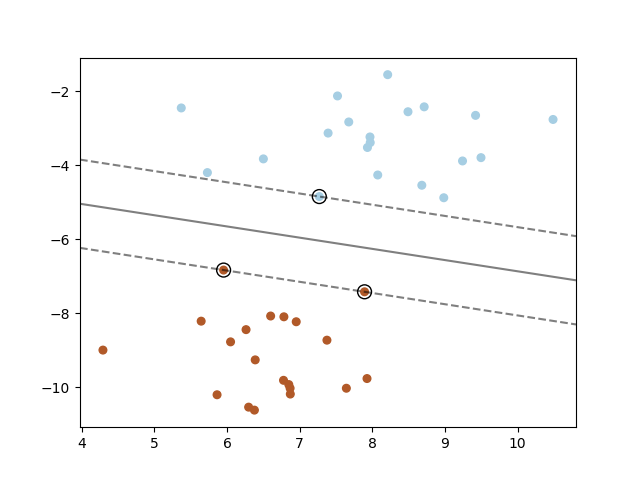
\includegraphics[scale=0.7]{images/intro-images/SVM_example.png}
   \caption{Support vector machine with training data visualized. 
   Blue and brown dots represents two different classes. 
   Circled points represent the support vectors. The dashed lines are all linear combinations of these support vectors. 
   The solid line represent the hyperplane splitting the two classes. The dashed lines can also be interpreted as the margins between the support vectors and the hyperplane.}
   \label{fig:svm_example}
\end{figure}

\subsubsection{Data separability}
Linear models are models made for linear data. In two dimensions linear models want to find trends in the data in accordance with a line. As mentioned above, a SVM is a linear model that finds separating hyperplanes as tools for making predictions. 
\par If the data isn't linearly separable\footnote{data is rarely linearly separable in practice \cite{Flach:2012:MLA:2490546}}, there exist no linear hyperplane that completely separates the two classes \cite{Flach:2012:MLA:2490546}. Figure \ref{fig:svm_example} visualizes a completely separable training data, as the brown dots can be separated from the blue dots with a line (e.g. the solid center line). Data that cannot be separated by a line might still follow a linear trend. \textit{Outliers} may make the data inseparable. An outlier is a point among data whose features describe a class in an unusual way. An outlier could simply be a point that have been miss-labeled by accident \cite{Flach:2012:MLA:2490546}. Using the example classes above, an outlier could be an 'apple' that looks like a 'car'.
\par To counter outliers and generally make support vector machines applicable to almost separable training-data, \textit{slack variables} was introduced to SVMs and the concept of soft-margin/hard-margin SVMs was established \cite{Cortes:1995:SN:218919.218929}.

\subsubsection{Soft-margin SVMs}
\par For linearly separable data sets there exists an infinite amount of possible decision functions, but only one is optimal. For inseparable data the selection of the decision function is decided by the user parameter traditionally referred to as the C-parameter \cite{Cortes:1995:SN:218919.218929} (complexity variable) or \textit{slack} variable. The C-parameter is a constant which allow for some some points to be miss-labeled during training. When allowing for a lot of slack (setting a low value to the C-parameter), more points are allowed on the wrong side\footnote{Also known as margin violations \cite{Flach:2012:MLA:2490546}} of the hyperplane and a larger margin is obtained. How changes to the C-parameter could impact a soft-margin SVM on almost separable data are visualized in Figure \ref{fig:svm_soft_example} and Figure \ref{fig:svm_harder_soft_example}.

\par The creation of the decision boundary based on the available training data is normally defined according to Equation \ref{eq:decision}. Based on the weights and feature-values in vector $x$, introducing slack $\epsilon$ into the equation a tolerance is added which re-define Equation \ref{eq:decision} as follows:

\begin{equation}\label{eq:soft_decision}
    w \cdot x > 1 - \epsilon. 
\end{equation}

\par SVMs that do not use slack variables (or that use a very high C value e.g 1e10)  are referred to as hard-margin SVMs. Contrary to soft-margin SVMs, a hard-margin SVM requires the training data to be completely linearly separable \cite{Cortes:1995:SN:218919.218929}.

\begin{figure}
\centering
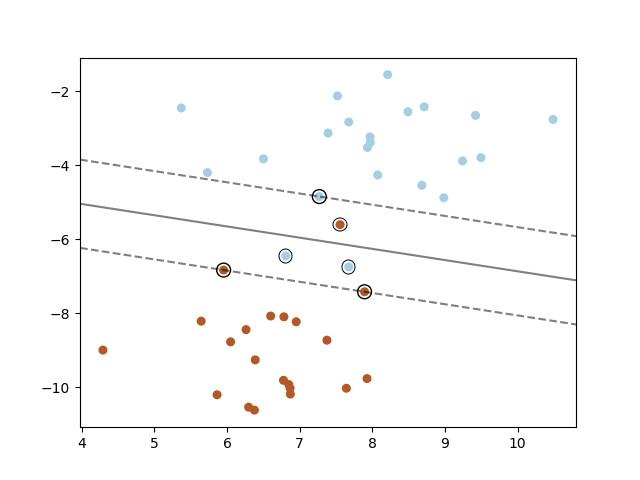
\includegraphics[scale=0.7]{images/intro-images/SVM_example_soft.png}
   \caption{Soft margin SVM. Compared to Figure \ref{fig:svm_example} a data set that normally would be inseparable, could still be solved with a soft margin SVM.}
   \label{fig:svm_soft_example}
\end{figure}

\begin{figure}
\centering
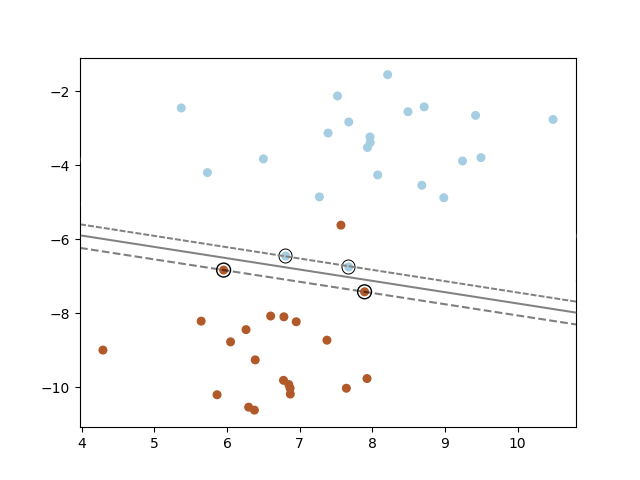
\includegraphics[scale=0.7]{images/intro-images/SVM_example_soft_harder.png}
   \caption{If a higher value is set to the C-parameter, a narrower decision boundary is drawn As a result the model has fitted to the training data better, but might generalize less as a result.}
   \label{fig:svm_harder_soft_example}
\end{figure}


As mentioned above, soft-margin SVMs were meant to solve the problem of not being able to train on data with the smallest of errors in \cite{Cortes:1995:SN:218919.218929}. When soft-margin SVMs do not suffice, other methods to extend their functionality have been employed such as kernel tricks.

\subsubsection{Kernel tricks}
\begin{figure}
\centering
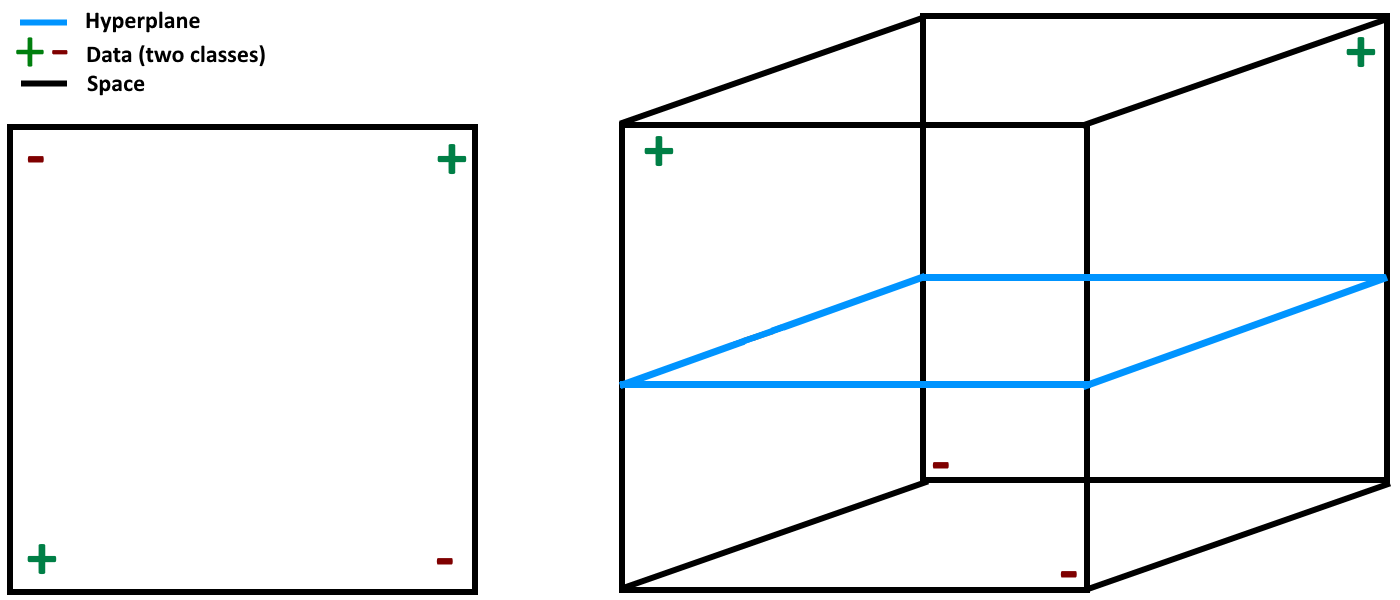
\includegraphics[scale=0.35]{images/dimred_images/kernel2d3dplane2.png}
   \caption{Concept of a kernel. The data visualised in the left side image, is representing a data set of four points in a two dimensional plane, (can be considered as clusters of points) that are non-linearly separable. There is no way of drawing a line that partitions the two classes separately. With a kernel, a third axis is simulated to transform the data into what is visualised in the right side image. As one can clearly see, the data in the right side image is linearly separable by the hyperplane portrayed in blue.}
   \label{fig:kernel}
\end{figure}

\par Data that is too noisy and non-linear in its nature can be transformed into something completely linearly separable by using what is called a kernel trick \cite{Flach:2012:MLA:2490546}. In a way, a kernel is considered to be a function that manipulates and/or adds information to the feature space based on the input space (the raw input data) to transform the data into something desirable by the model \cite{Flach:2012:MLA:2490546}.

\par A visualisation of what a kernel could achieve can be seen in Figure \ref{fig:kernel} and Figure \ref{fig:kernel2}. A hyperplane is visualised in light blue. The left side \textit{boxes} have no way of separating the green plus-signs from the red minus-signs with a linear plane. How ever, the right side images clearly show that increasing the dimension and offsetting the data along and additional axis would make the data linearly separable. The examples are not constructed based on real kernels, the Figures are merely explanatory.



\begin{figure}
\centering
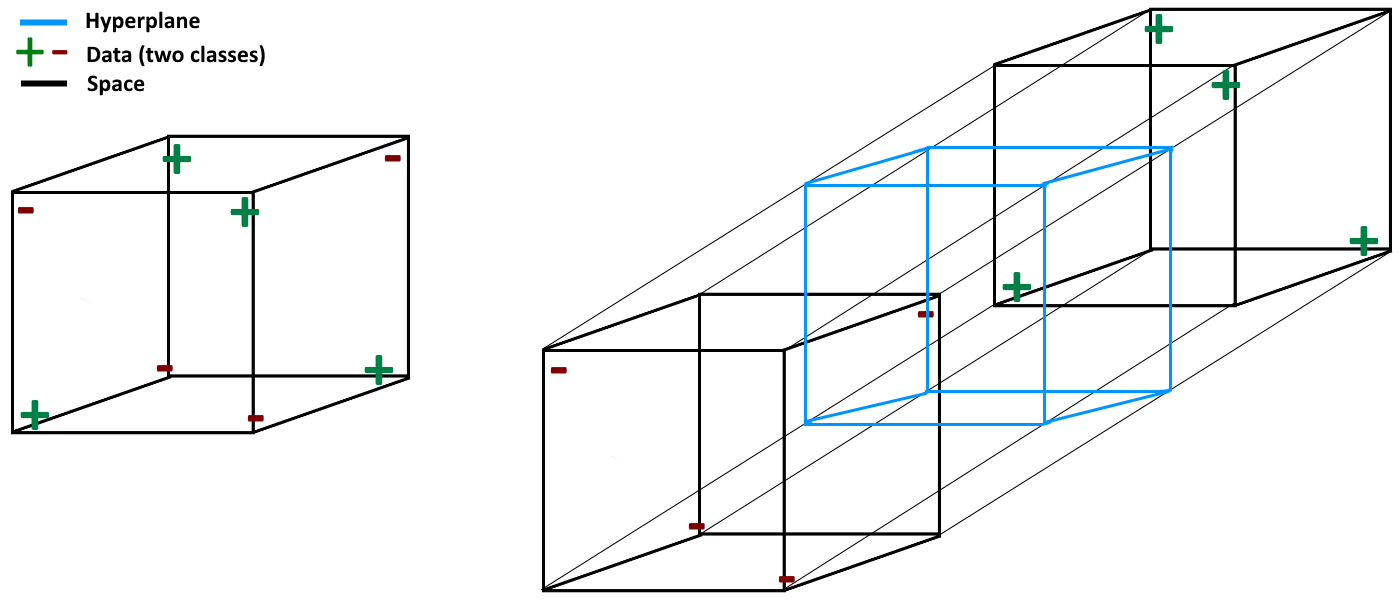
\includegraphics[scale=0.35]{images/dimred_images/kernel3d4dplane.png}
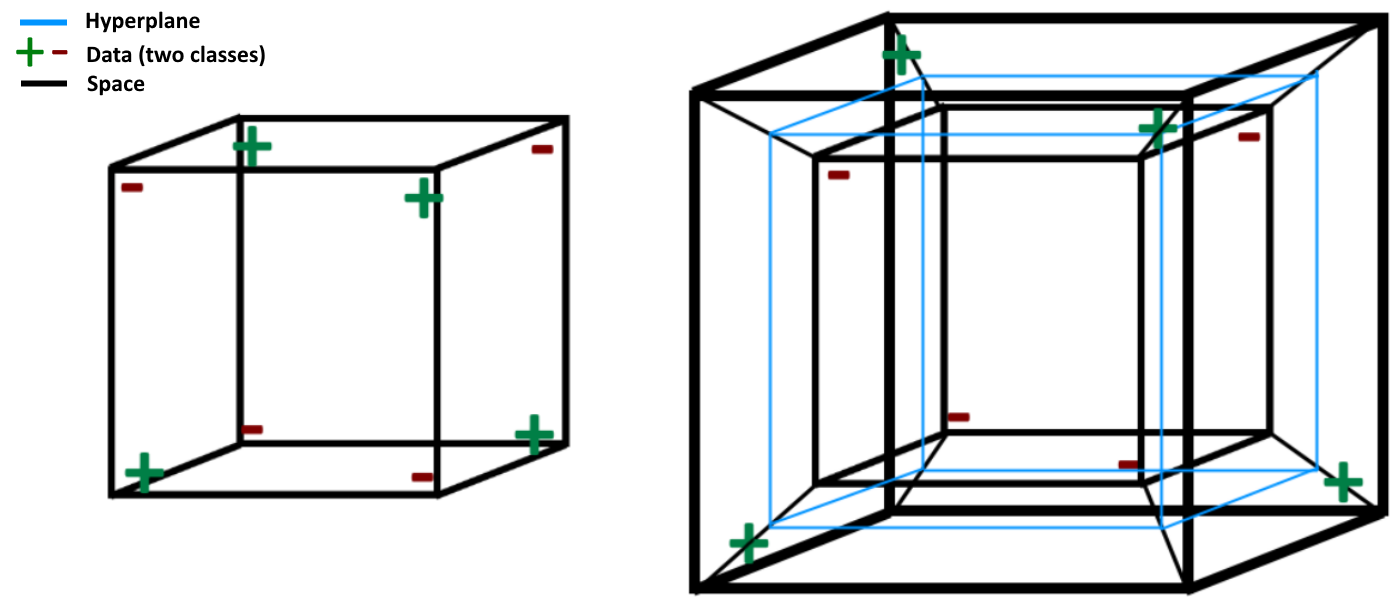
\includegraphics[scale=0.35]{images/dimred_images/kernel3d4dpottplane3.png}
   \caption{Two similar visualisations to Figure \ref{fig:kernel}, instead going from 3D to 4D to make data linearly separable by a plane (that in the fourth dimension is three dimensional (therefore visualised with a blue cube)). }
   \label{fig:kernel2}
\end{figure}



\section{Hyperplane Folding}
Lundberg et al. \cite{unpublished} experimented with a method that rotates (or folds) data based on the intersection between hyperplanes from two separate support vector machines trained on two separate parts of the same training data set. The proposed method was coined \textit{Hyperplane folding} (in this paper, HPF for short). The results in the study clearly showed that the margin in a SVM had the potential to increase, having used HPF to not having used HPF. How ever, some weaknesses come with the method that could be fatal for some cases in the algorithm, particularly during classification. HPF also demonstrate potential for handling non linear data. Unlike an applied kernel trick, HPF works similarly to a piecewise linear SVM (PWL-SVM) \cite{PWLSVM}. Both HPF and PWL-SVM could be used in combination with kernels, but adds an extra ability to handle non-linearity. For instance, a kernel may merely improve the geometry of the data, and then be finished into a fully functioning linear model using PWL or HPF. More detail in how Hyperplane folding works will be mentioned in the next chapter of the thesis. 

\par The study presented in this thesis serves as an extension to the original HPF in an attempt to solve some of HPFs weaknesses. We call the primary extension \textit{Rubber band folding} (RBF), which is used to prevent an over-rotation that can happen during classification when using HPF. We believe in the investiation of HPF as we agree with \cite{PWLSVM} that states that non-linear classifiers are requiered as linear classifications capability is too limited for real life applications. The study will compare HPF method improved with Rubber band folding to the original HPF method and to a state of the art SVM solution from \textit{sci-kit learn} \cite{scikit-learn}.

\section{Research questions}

\begin{enumerate}
  \item To what extent does Rubber band folding increase the margin of the Support vector machine.
  \item Can Rubber band folding improve the classification accuracy of Hyperplane folding? 
  \item How will the total execution time of the system increase when Hyperplane folding is used.
\end{enumerate}


\chapter{Related work}
\par Hyperplane folding was first mentioned in  \cite{unpublished}. Where the primary support vector was used as delimiter to split the data. In the general case for two dimensions, a trained model has three support vectors. The primary support vector is in that case the support vector 'from the class with only one support vector' \cite{unpublished}. The method rotated all data points in one of the split sets by a fixed angle. The original implementation was also only applied to three dimensions at most and only completely separable data.

\par Similarly  \cite{PiotrRandomRotation} rotated the feature space, but for each individual base-learner in tree-ensembles. Rotating data can be applied as a pre-processing technique to introduce more diversity into the data, which often is desirable for ensemble learning. Unlike  \cite{unpublished}, the rotations were applied in dimensions higher than two and rotated data at random and only prior to learning. Contrary Hyperplane folding \cite{unpublished} require its data to be rotated before attempting its predictions.

\par Belkin and Niyogi \cite{Belkin:2003:LED:795523.795528} developed a method using \textit{Laplacian Eigenmaps} where the end goal was to lower the number of dimensions needed to represent data. Sometimes the size of the feature space is unnecessarily large where using a lower dimensional manifold would both yield a similar result meanwhile being more interpretable. A k-NN algorithm was used to reduce the features.

\par A method similar to the one presented in this paper (and by \cite{unpublished}) that handles non-linear data with SVM are piecewise linear support vector machines (PWL-SVM). \cite{PWLSVM} divide data much like \cite{unpublished} with the HPF mathod. Each divide, which there can be several of, uses its own decision boundary contrary to HPF which rotates one side to merge the hyperplanes.

\par Breiman \cite{hingeplane} merged hyperplanes using a hinge functions. Sums of hinge functions could be used to construct predictors that are accurate for non-linear multivariate data in regression tasks. Related to \cite{unpublished} hyperplane folds, multiple hinge function yield improved results where more hinges approximates the decision function better.

\par Koggalage and Halgamuge \cite{reducetraining} wanted to reduce the amount training samples to improve the training time for SVMs by removing unnecessary samples. The simple premise was, that removing anything but support vectors will have no effect on the end result. Therefore training samples far away from the decision boundary will naturally be less probable to be a support vector. Using crip-clusters and distance based safety regions whole areas where data consisted of just one label are discarded. Clusters were identified using K-mean which are faster than SVMs.

\par Park and Sklansky wanted to minimize the number of Tomek links required to fit a multi-class regression classifier\cite{parksklansky}. The links were later approximated with a hyperplane that aimed at cutting as many links as possible, iteratively cutting more links. Cutting more links ensures less hyperplanes are needed. They found that using more links yielded a better error rate. Tenmoto et al. later supplemented Park and Sklanskys approach in \cite{tenmoto}. They aimed at improving the selection of hyperplane. Instead of iteratively finding a better hyperplane among all links, they added more links in succession as an alternative way. 

\chapter{Hyperplane folding}

\section{Existing technique}

\par Hyperplane folding, first proposed by Lundberg et al. \cite{unpublished}, increases the margin between classes, by rotating partitions of the data depending on the results of applied support vector machines. 
\par Hyperplane folding splits the training data by locating the \textit{Primary support vector} \cite{unpublished} and then having a line pass through it, in the direction of the weight vector of the support vector machine.
\begin{figure}
\centering
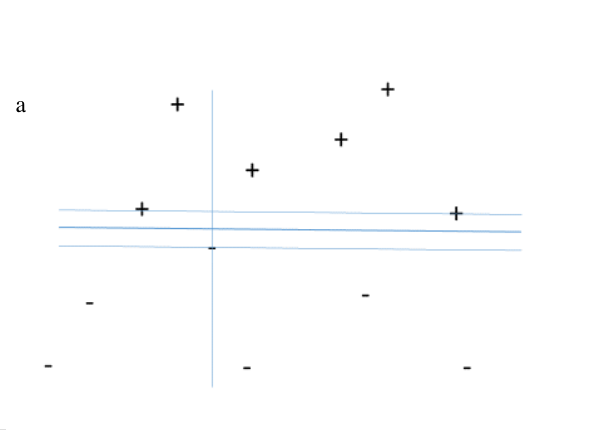
\includegraphics[scale=0.7]{images/intro-images/hpf_1.png}
   \caption{Initial state of the Hyperplane folding algorithm. The primary support vector has been located, which is illustrated by the vertical line.}
   \label{hpf_1}
\end{figure} 
The primary support vector is illustrated in Figure \ref{hpf_1}. The line is used to create two sets, one set for each side of the line. The support vector machine algorithm is then applied on both sets, creating two new hyperplanes with two new margins where the lowest of the two margins, will either be higher or equal to the original SVMs margin \cite{unpublished} as can be seen in Figure \ref{hpf_2}.
\begin{figure}
\centering
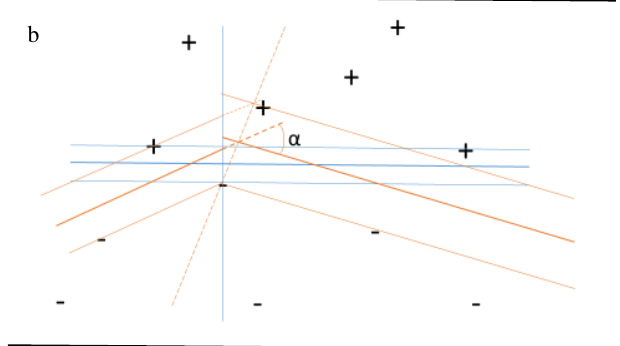
\includegraphics[scale=0.7]{images/intro-images/hpf_2.png}
   \caption{Two support vector machines has been created, and their margins are illustrated by the orange lines. }
   \label{hpf_2}
\end{figure} 
\par By merging the two hyperplanes into one, the lowest margin of the two new Support vectors machines will as a result be the new margin for the training data. Merging is done by rotating the data in one of the two sets by the intersection angle between the two hyperplanes. This results in a new support vector machine that has higher or equal margin to the original support vector machine \cite{unpublished}. The rotation process is seen in Figure \ref{hpf_3} and the result of the hyperplane folding algorithm in Figure \ref{hpf_4}.

\begin{figure}
\centering
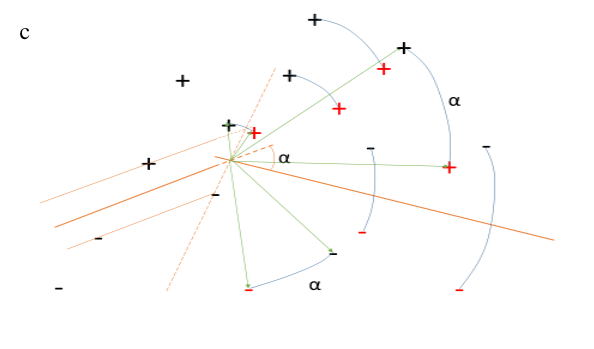
\includegraphics[scale=0.7]{images/intro-images/hpf_3.png}
   \caption{The SVM with the highest margin is rotated by the intersection angle, in order to align it and its data points to the other SVM. }
   \label{hpf_3}
\end{figure}
\par During classification of points (predicting labels of unknown points using a fit model) the unknown data must undergo the same pre-processing-procedure as the training data was subjected to during training. This is firstly done by determining whether or not, points reside in the same space that got rotated during training. E.g. Determine what side of the primary support vector\footnote{More accuratly stated, what side of the line that goes in the direction of the normal through the primary support vector.} the points are located\footnote{Visualized as, a point located to the left or to the right right of the dotted line in Figure \ref{fig:hpf_pre_rotation}.}. If a point lies in the side that was rotated during training, the point must be rotated by the intersection angle prior to classification. 

\par The process of splitting and rotating the hyperplanes could be repeated in order to improve the margin further \cite{unpublished}.
\ref{hpf_4}
\begin{figure}
\centering
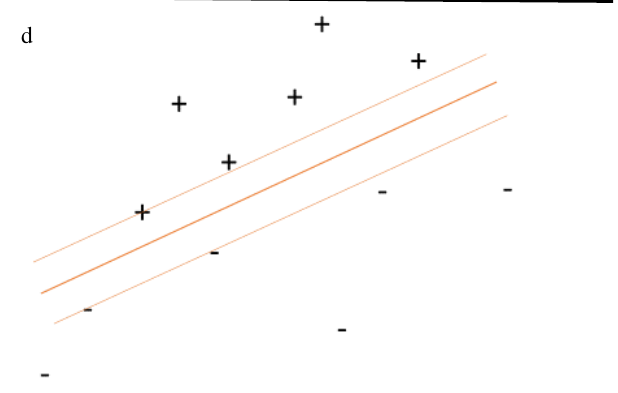
\includegraphics[scale=0.7]{images/intro-images/hpf_4.png}
   \caption{A new SVM has been created with a margin greater or equal to the inital support vector machine.}
   \label{hpf_4}
\end{figure}

\par At most the folding process is repeated until there are only two support vectors, as a support vectors machine with two support vectors is the optimal case. Applying Hyperplane folding when only two support vector are present could cause one of the disjoint sets to only have data points from one class, from which it is not possible to form a support vector machine from.

\subsection{Current limitations}
Hyperplane folding is limited to the two dimensional case (featurespace of size two), which requires data in higher dimensions to be projected prior to training. The projection serves as a dimensionality reduction and is described more in detail later in the thesis. 
\par Another limitation of hyperplane folding is that data sets are required to be linearly separable in order to guarantee a correct fold. As soft margin / non-linearly separable data sets have outliers that potentially could be disregarded and/or included incompatibly by the two separate SVMs that generate the folding hyperplanes.
\par Further the algorithm is limited to binary (two classes) classification.
\par Classification of unknown datapoints positioned in certain areas will always be miss classified when hyperplane folding is used.
\par These limitations will be elaborated on further.


\subsection{Problem Description}
\label{Problem description}
\begin{figure}
\centering
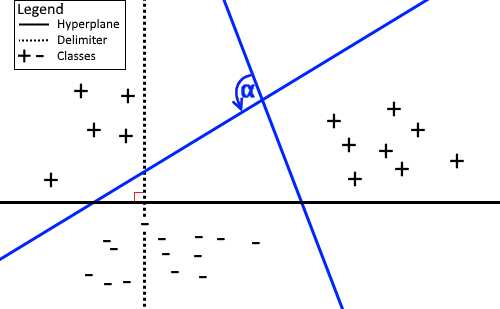
\includegraphics[scale=1]{images/intro-images/hyperplaneExplanation1_6.png}

   \caption{Hyperplane folding: The black horizontal hyperplane is part of the SVM that is initially trained on all data and is used to find the primary support vector (for the delimiter). The dotten line is the delimiter, which goes in the direction of the normal to the original hyperplane through the primary support vector. The blue hyperplanes belong to the new SVMs, trained on their corresponding split. Data points on the right side of the delimiter (the SVM with largest margin) can be rotated around the intersection point with the intersection angle to align the blue hyperplanes.}
   \label{fig:hpf_pre_rotation}
\end{figure}
As previously mentioned the hyperplanes are dependent on their support vectors. Rotating the data (including the support vectors) around the intersection point therefore rotates the hyperplanes. By rotating the point with the intersection angle, as performed by \cite{unpublished}, aligns the two hyperplanes. In Figure \ref{fig:hpf_pre_rotation} the vertical dotted line indicates a delimiter that passes through the \textit{primary support vector}. The delimiter split the data into two disjoint sets. The algorithm then duplicates the primary support vector into both disjoint sets\footnote{Which actually makes them not disjoint anymore.}. In Figure \ref{fig:hpf_post_rotation} the data points to the right of the delimiter have been rotated because the disjoint data set on that side had generated a SVM with a slightly larger margin \cite{unpublished} than the one to the left side of the delimiter.

\begin{figure}
\centering
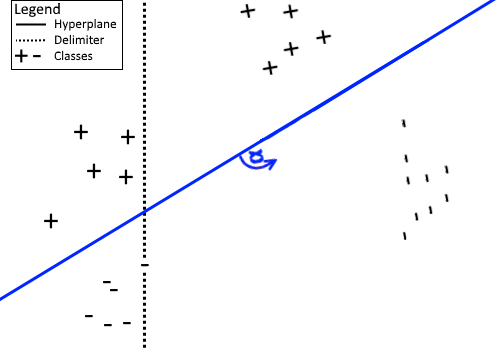
\includegraphics[scale=1]{images/intro-images/hyperplaneExplanation2.png}
   \caption{Post rotation, the hyperplanes are aligned. The primary support vector have been duplicated.}
   \label{fig:hpf_post_rotation}
\end{figure}

\par A problem arises when classifying unknown data points. Depending on the points position in the hyperspace, they must be rotated in accordance with the rules that the training-data was rotated. This rotation could cause a point to be rotated to the other side of the hyperplane and as a result be incorrectly classified. This is illustrated in Figure \ref{fig:hpf_weakness}, where the positive sample in purple must be rotated with the same angle as the right side training-data were. Since the rotation is applied around the intersection point, the purple point will end up on the wrong side of the hyperplane and be labeled as belonging to the negative class.
Rotating a point to the other side of the hyperplane is undesirable for obvious reasons and is also the reason to why hard-margin SVMs must be used. With a soft margin SVM outliers could potentially be rotated to the wrong side of the hyperplane even during the training phase.


\begin{figure}
\centering
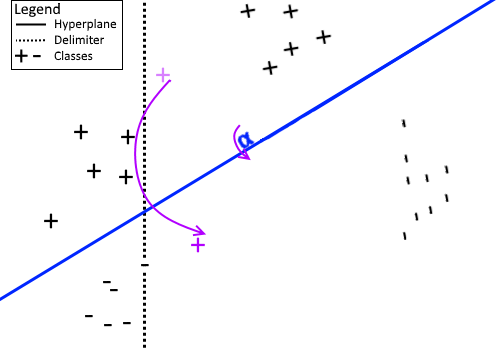
\includegraphics[scale=1]{images/intro-images/hyperplaneExplanation3.png}
   \caption{Hyperplane foldings weakness: During classification a positive sample located as illustrated in purple get rotated below the new hyperplane.}
   \label{fig:hpf_weakness}
\end{figure}

\par This thesis purpose was to solve some of the above mentioned limitations and problems that are present in the existing Hyperplane folding technique. To extend Hyperplane foldings capabilities, Rubber band folding was researched. 

\section{Improving Hyperplane folding with Rubber band folding} 

Lundberg et al. \cite{unpublished} mostly worked with the general case of having three support vectors present in a SVM trained on two dimensional data. Therefore the support vector belonging to the class with only one support vector was selected as the primary support vector. For cases when more support vectors are generated, another method for selecting the primary support vector is needed.
\subsection{Selecting the primary support vector}

\par Some data sets will have generated more than three support vectors. This case can arise in particular after having projected data into two dimensions. This is due to the fact that computers have limited resolution \cite{unpublished}. Because of the resolution problem both classes may have more than one support vector\footnote{For example four support vectors with two in each class.} when in two dimensions. When more support vectors are present a non-trivial case is introduced, when selecting the primary support vector. Selecting the primary support vector as the support vector from '... the class with only one support vector' \cite{unpublished} would simply be impossible having no class with only one support vector.

\subsubsection{Support vector traversing}
\par The support vectors for each class will be a linear of combination of the hyperplane, regardless of the how many support vectors are present. By traversing the support vectors in order, starting with the most distant support vector (with the lowest x value), the primary support vector will be the the first support vector that is of the other class. This will ensure that the split result in two new Support vector machines that are guaranteed to intersect. Without an intersection a fold is not possible. 
\begin{figure}
\centering
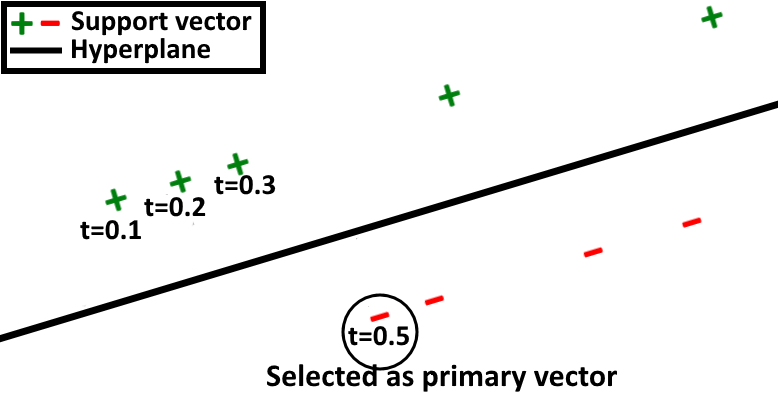
\includegraphics[scale=0.6]{images/intro-images/primaryvec2.png}
   \caption{Selecting the primary vector. The $t_k$ value increase as a point progress upwards in the direction of the hyperplane. As a positive sample is most distant (lowest $t$-value, the first minus sign will be chosen to be the primary support vector when traversing.}
   \label{fig:traverse}
\end{figure}



\par Finding the primary support vector require for the support vectors to be sorted by their occurrence in the hyperspace along the direction of the hyperplane. This is done by projecting the support vectors onto the decision function and calculating a t-value, which is a scalar that ranks a point based on its position along the decision function. This is achieved using the parametric description for the projection of a point onto a two dimensional plane in Equation \ref{eq:parametric}. Where $(x_k, y_k)$ is a point in the hyperspace being projected onto the line $(a,b)$ and $(c,d)$ is a point on the line.
\par Projecting a point in the hyperspace orthogonally onto the line, could be interpreted as moving the point towards the line in the direction of the normal of that line. The normal of the line could be derived from its equation into $b,-a$. From that follows that offsetting the point in the direction of the normal scaled by $s$ yield a point on the line. As $t$ represents a unit of length for a point on the vector, solving $t_k$ in Equation \ref{eq:parametricproj} gives unit of length for point $k$. The larger value $t$ acquires, the further to right the point is positioned on the line.  Solving for $t_k$ in Equation \ref{eq:parametricproj} gives the algorithm for solving this problem which can be seen in Equation \ref{eq:tk}.
\begin{equation}\label{eq:parametric}
\begin{aligned}
   \begin{cases}
    x = at + c \\
    y = bt + d
    \end{cases}
\end{aligned}
\end{equation} 

\begin{equation}\label{eq:parametricproj}
    \begin{aligned}
        \begin{cases}
            x_k + bs = at_k + c \\ 
            y_k - as = bt_k + d
        \end{cases}
    \end{aligned}
\end{equation} 

\begin{equation}\label{eq:tk}
    t_k = \frac{a(x_k - c) + b(y_k - d)}{a^2 + b^2}
\end{equation}

Compiling a list of all support vectors sorted ascending by their $t_k$  value yields a list where the support vectors are sorted by their occurrence from left to right. By selecting the first support vector  and it's class in the list, it is possible to traverse the list and finding the primary support vector. As it will be the first support vector to the right of the initial support vector residing in the other class. In psudo, Algorithm \ref{al:traverse} achieves this. Illustrated in Figure \ref{fig:traverse} is a made up example of many support vectors lying next to a hyperplane. 

\begin{algorithm}[H]\label{al:traverse}
 \KwData{Support vectors with their corresponding class}
 \KwResult{Primary support vector}
 
 \ForEach{vector in support vectors}
 {
  tk.Append(calculateT(vector))
 }
 tk.Sort()\\
 
 firstClass = tk[0].vec.class

 \For{t in tk}{
    \If{firstClass != t.vec.class}{
        return t.vec.class
        }
 }
 \caption{Finding primary support vector}
\end{algorithm}

\subsection{Splitting the data}
When the primary support vector has been found, the data is split by creating a two dimensional plane using the normal of the original hyperplane as a direction and the primary support vector as origin. This creates a splitting hyperplane, where any points above the plane will belong to the right set, and any points bellow the plane will belong to the left set. This splitting hyperplane will be diagonal in it's relation to the hyperspace, and therefore encapsulate larger areas of the space, reducing the risk of splitting the data set in such manor that only one class will reside in either of the two resulting sets. This line is created by creating a vector $v$ going from the primary support vector to the point that is being evaluated. If the dot-product between the hyperplanes direction and v is greater than 0, the point resides in the right set, if smaller than 0 it resides in the left set. Equation \ref{eq:split} illustrates the mathematics of the split.
\par The primary support vector will by definition reside in both sets, as the splitting hyperplane imposes a equal or greater than equality when assigning the data points to the sets. This will in turn introduce a new data point / duplication of the primary support vector, where one of the copies will remain in its original position, and one will be rotated accordingly to the fold.
\begin{equation}\label{eq:split}
\begin{aligned}
    v = (P_x, P_y) - (PS_x, Py) \\
    h = (-W_y, W_x) \\
    h = v \cdot w \\
\end{aligned}
\end{equation} 



\subsection{Rubber band folding}

\begin{figure}
\centering
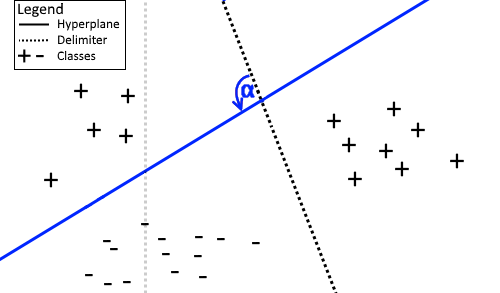
\includegraphics[scale=1]{images/intro-images/rubberbandExplanation1.png}

   \caption{Using Hyperplane folding with Rubber band folding, the steps visualized in Figure \ref{fig:hpf_pre_rotation} are performed to generate the two hyperplanes and the angle alpha. After that a new delimiter is drawn (previous delimiter displayed faded), that is defined by one of the two hyperplanes. The data is re-partitioned depending on what side the new delimiter they reside on.}
   \label{fig:rbf_pre_rotation}
\end{figure}


Once the data has been split two new classifiers are generated, one for each split. According to the previous method presented in \cite{unpublished}, the data in one of the two splits get rotated by the angle between the two decision functions around the intersection point (intersection between the two decision-functions). The previous method is visualized stepwise in Figure \ref{fig:hpf_pre_rotation} going to Figure \ref{fig:hpf_post_rotation}. As previously mentioned, problems during the classification-step arise when using this method.

\par \textit{Rubber Band Folding} is a method that extends the previous Hyperplane folding method. Both methods works similar in how the data is split into two parts. It is after having found the intersection point and angle between the two separate decision boundaries that Rubber band folding differ itself from the previous method.

\par The actual region that get rotated have changed. Instead of using the data at one side of the original hyperplanes normal passing through the primary support vector, e.g. left or right of the delimiter (dotted line) in Figure \ref{fig:hpf_pre_rotation}, an additional split is made. The new split separates data with the hyperplane belonging to the SVM trained on the side of the data that should be rotated. 
\par In Figure \ref{fig:rbf_pre_rotation} the delimiter performing the first split is displayed as faded. Compared to Figure \ref{fig:hpf_pre_rotation} the new delimiter is the hyperplane belonging to the right side.

\par Two important things to note about Rubber band folding. Firstly it does not matter what side of the first split get rotated. Contrary to the correct implementation of previous method proposed by \cite{unpublished}, where the side with the largest margin is rotated, which side of the data that get rotated is now irrelevant. Secondly the new split is applied to all data and not just the side that gets rotated. A misconception is that two splits are made in sequence, making three sections. Rather the data is merged back together after the first split, having found the intersecting hyperplanes and angle, then another split is made to all data using a new delimiter. What the new split achieves may be more clear if you imagine Figure \ref{fig:rbf_pre_rotation} without the dimmed dotted line.

\par The new split ensures that points can not be rotated below the hyperplane since what is rotated is already above the right side hyperplane.




\subsubsection{Calculating the intersection point}
\par The two hyperplanes are guaranteed to intersect thanks to the primary support vector. What remains are finding the intersection point and the intersection angle.

\par The intersection point is calculated by solving Equation \ref{eq:intersection_1}, for $x$ and $y$, resulting in equation \ref{eq:intersection_2} where the steps have been reduced. The rotational angle, omega, is then given by solving equation \ref{eq:rotationangle}.
\begin{equation}\label{eq:intersection_1}
\begin{aligned}
   \begin{cases}
    a_1 x + b_1  y + c_1 = 0 \\
    a_2 x + b_2 y + c_2 = 0 \\
    \end{cases}
\end{aligned}
\end{equation} 
\begin{equation}\label{eq:intersection_2}
\begin{aligned}
   \begin{cases}
    \cfrac{b_1 c_2 - b_2 c_1}{a_1 b_2 - a_2 b_1}  = x \\
    \cfrac{a_2 c_1 - a_1 c_2}{a_1 b_ 2 - a_2 b_1} = y\\
    \end{cases}
\end{aligned}
\end{equation} 

\begin{equation}\label{eq:rotationangle}
\begin{aligned}
   \begin{cases}
    \omega = arccos \cfrac{a_1 a_2 + b_1 b_2}{\pm \sqrt{(a_1^2 +  b_2^2) (a_2^2 + b_1^2)}}
    \end{cases}
\end{aligned}
\end{equation} 

From $\omega$ the two dimensional rotation matrix in Equation \ref{req:rotationmatrix} is formed. Technically the $arccos$ term in Equation \ref{eq:rotationangle} is unnecessary, as the cosine of alpha is used to form the rotation matrix. Instead the sinus part of the matrix could be found from the Pythagorean trigonometric identity $sin(\omega) = 1 - cos(\omega)^2$. 
\par Consider $\omega$ in radians for explanations below.


\begin{equation}\label{req:rotationmatrix}
{
\left({\begin{array}{ccc} cos(\omega) & -sin(\omega) \\ sin(\omega) & cos(\omega) \end{array}}\right) 
}
\end{equation}

\par The rotation is applied around the intersection point. Therefore points coordinates $(x_i, y_i)$ must be translated to the origin before rotating. After having rotated the points according to Equation \ref{req:rotationmatrix} they must be translated back the same distance. This defines the rotation function for Hyperplane folding as can be seen in Equation \ref{req:applyrot}. 


\begin{equation}\label{req:applyrot}
{
\left({\left({\begin{array}{ccc} cos(\omega) & -sin(\omega) \\ sin(\omega) & cos(\omega) \end{array}}\right) 
\left({\begin{array}{c} x_i - x \\ y_i - y \end{array}}\right) +
\left({\begin{array}{c} x,  y \end{array}}\right) 
}\right)}
\end{equation}


\subsubsection{Rotation constraint}
\par In addition to the new split a constraint is added to the rotation as part of the Rubber band folding extension. The constraint is visualized in Figure \ref{fig:rbf_classification}. 

Instead of always rotating points by the intersection angle, they follow a condition seen in Equation \ref{eq:rubberbandangle}. $\alpha$ is the intersection angle between the two hyperplanes and $\beta$ is the angle between the point and the normal of the plane that is not going to be rotated.

\begin{equation}\label{eq:rubberbandangle}
\begin{split}
    \omega = min(\alpha, \beta)
\end{split}
\end{equation}

\par This eliminates a problem that could potentially lower the margin. If the purple point in Figure \ref{fig:rbf_classification} would be rotated by $\alpha$ (the dimmed arrow) the margin would be lowered, which is something this thesis work want to improve.

\subsection{Termination state}
When the new classifier has two support vectors, one for each class, the folding stops as the optimal classifier for the data set has been found \cite{unpublished}. The algorithm in two dimensions can be summarized as in Algorithm \ref{al:hyperplaneoverview}. However, due to floating point precision errors, the algorithm should be aborted when the margin increase between folds are less than a specified threshold, $\epsilon$. 
\par It is also possible to manually specify the maximum number of folds to perform before terminating.
\begin{figure}
\centering
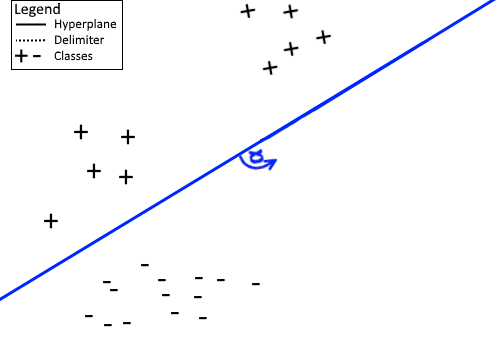
\includegraphics[scale=1]{images/intro-images/rubberbandExplanation2.png}

   \caption{Post rotation having used Rubber band folding. Compared to Figure \ref{fig:hpf_post_rotation} the negative points remain untouched, having used Rubber band folding.}
   \label{fig:rbf_post_rotation}
\end{figure}

\begin{algorithm}\label{al:hyperplaneoverview}
 \KwData{Trained support vector machine with a data set with labels}
 \KwResult{Hyperplane folding classifier}
 
\While{numberOfSupportVectors > 2 or marginChange < $\epsilon$ or numberOfFolds = maxFolds}{
    findPrimarySupporVector()\\
    divideData() \\
    rotatePointsInRotateSet()\\
    overwriteWithNewSVM()
}
 \caption{Overivew of Hyperplane folding}
\end{algorithm}

\subsection{Classifying datapoints}
\par During the training process, intersection points, hyperplane normals, intersection angles and primary support vectors are stored into a list for each fold. These are stored to perform the classification step.
\par When classifying unknown data points, folds that were applied to the training data must be applied in the same manor to the unknown data. The folds are replicated from the information in the list. 
\par Initially the process identifies whether or not the point should be rotated. This is done by locating the splits from the primary support vector, hyperplane normal and the splitting point.
\par If the point is located in an area that was rotated during training, then it is rotated based on the angle and intersection point using Equation \ref{req:applyrot}.



\begin{figure}
\centering
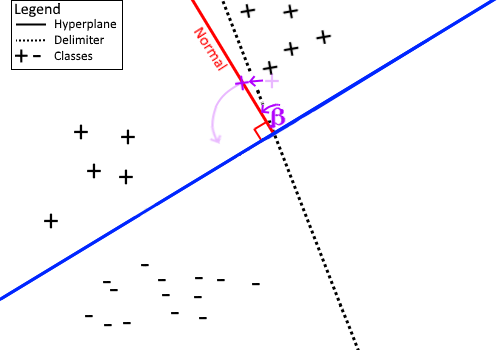
\includegraphics[scale=1]{images/intro-images/rubberbandExplanation3.png}

   \caption{Rubber band folding used during classification of a unknown point. The maximum angle which the purple point can be rotated by is beta. Beta is decided by the normal of the plane that is not rotated. If beta is less than alpha (the intersection angle), beta is used to rotate the point instead of alpha. This will result in points lying on the normal-line. The faded curved arrow in purple illustrate where the point would end up if it were to be rotated by alpha. As can be seen, rotating the point with alpha would give the undesirable result of a lower margin.}
   \label{fig:rbf_classification}
\end{figure}

%\section{Dimension reduction}
%As Hyperplane folding is limited to two dimensions, applying the algorithm on data sets with a feature space with higher dimensionality than two require preprocessing \cite{unpublished}. This paper introduces a technique that reduces the dimension of a data set two any dimension lower than the orginal dimension of the data set. This method is called Dimension reduction. 



\section{2D Projection}

\par The amount of available independent features in a data set defines its dimensions\cite{Belkin:2003:LED:795523.795528}. Three features equates to a three dimensional data set. 
% (mathematically setting one of the coordinates to zero)
\par A three dimensional space may be depicted in two dimensions by ignoring the last coordinate. Setting the third coordinate to, for example, zero renders the axis ineffectual.  In contrary by adding a coordinate that for all points attain the same value, increases the dimensions without contributing with any new useful information about the data e.g. the relationship between points remain the same but an additional axis exist.

\par A projection is a mapping that transforms data to an alternative representation. Zeroing out components of vectors, can be considered as orthogonal projections. Consider the example of a orthographic projection from a 3-dimensional space onto a XY-plane. Multiplying all points with the following matrix essentially changes the basis from $R^3$ to $R^2$: 

\begin{equation}\label{eq:orthogonalproj}
{
\left({\begin{array}{ccc} 1 & 0 & 0\\ 0 & 1 & 0\\ 0 & 0 & 0 \end{array}}\right) 
\left({\begin{array}{c} x \\ y \\ z \end{array}}\right) =
\left(\begin{array}{ccc} x & y & 0 \end{array}\right) 
}
\end{equation}

\par Being able to project data is important for \textit{Hyperplane folding} because it is only applicable in two dimensions, as seen in \cite{unpublished}. Data of dimensions higher than two will require pre-processing, where the goal is to achieve a two dimensional representation of the support vector machine. The relationship within data must remain unchanged. Features can not simply be removed as the loss of data wouldn't be representative of the data set and could easily make the data inseparable. Therefore a simple orthogonal projection as seen in Equation \ref{eq:orthogonalproj}, that although projects the data onto a two dimensional plane, will not always achieve a representation that would work for Hyperplane folding. Instead another method is proposed to achieve a two dimensional representation of the SVM without loosing information when projecting the data. 
%The method presented in this paper is called \textit{Align}, and applies rotations on the data uniformly to preserve the information whist still achieving a two dimensional representation of the SVM.

\subsection{Align - Procedure for aligning support vectors}
A SVM is defined by its support vectors. In this paper the denotation of \textit{a SVMs dimensions} is defined by the size of the feature space, that is the number of coordinates, of that SVMs support vectors. Manipulating a SVMs support vectors changes the SVM. Projecting the data, including the support vectors, into a lower dimensional representation by using Align therefore lowers the dimensions of the SVM.

\par The SVM is projected by applying a rotation around the origin to all data points, including the support vectors, which leave the relationship within the support vector machine unchanged. I.e. after rotating the points they will lie at the same distance from the origin as well as from each other, compared to before having performed the rotation. In other words the support vectors will make up a decision boundary with a margin of equal size with or without the rotation. This is self evident but is mentioned to further clarify that a projected SVM (trained on rotated data) will output the same result, as long as the same rotations that were applied to the training data are applied to unknown points prior to classification.\todo{ref på detta stycket}

\par A rotation applied with a matrix can be reversed with its inverse. In the Align algorithm multiple rotation matrices are formed and multiplied together in a accumulative matrix.  When the algorithm terminates the accumulated matrix is used to transform the data points. The transformed data will serve as a two dimensional projection of the SVM and Hyperplane folding will be applicable to the transformed data. 
\par Note that after having performed Hyperplane folding on the projected data, the inverse of the accumulated matrix is used to re-project the data back into its original dimensionality. By stepwise projecting then using Hyperplane folding and finally re-projecting is the use of dimension reduction for Hyperplane folding in dimensions higher than two.

\subsubsection{Algorithm}
\par Align rotates all data points around the origin so that two support vectors from the same class \textit{aligns}. Two vectors are said to be \textit{aligned} if their coordinates are the same except for the last coordinate i.e. having different depths. 

\begin{figure}
\centering
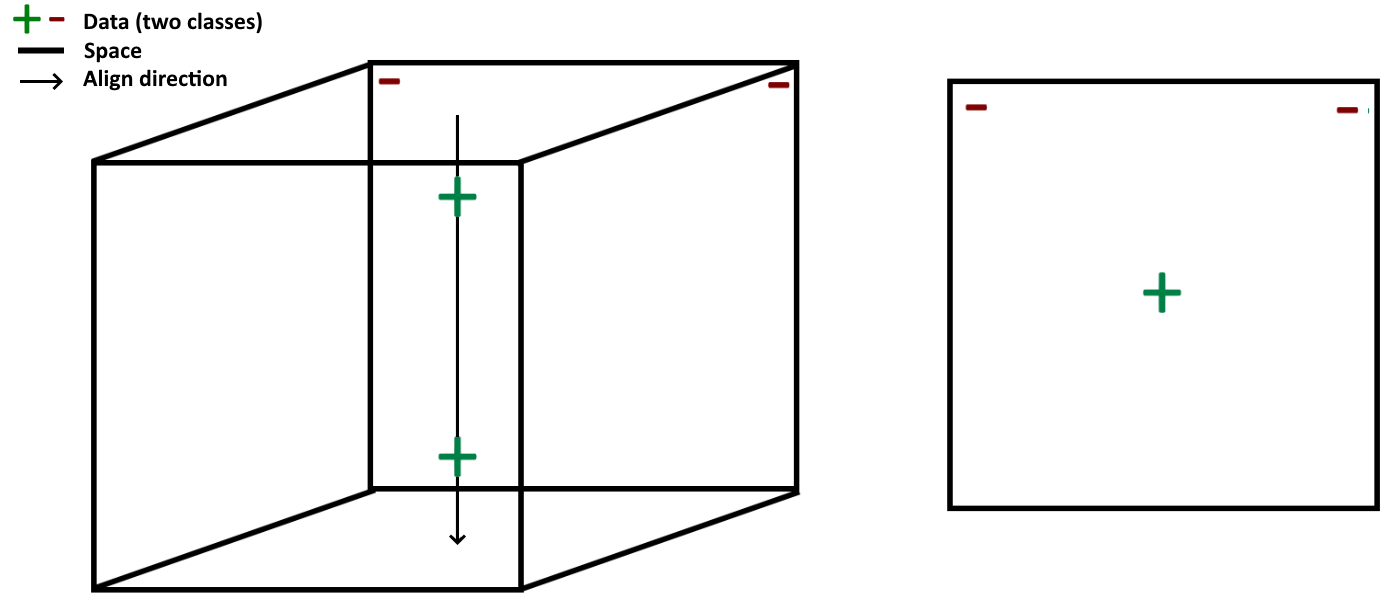
\includegraphics[scale=0.3]{images/dimred_images/align2.png}
   \caption{Visualisation of two (support) vectors being aligned. Where all four, two positive and two negative, points are support vectors in a three dimensional SVM (visualized as left cube). Rotating the box and aligning two vectors from the same class (in this case the + class) projects the SVM into two dimensions (visualized as right plane).}
   \label{fig:align}
\end{figure}

\par After two support vectors have been aligned, their last coordinate is disregarded to effectively serve as one and the same support vector in the SVM for all further projections/iterations on lower dimensions. After having projected the data one dimension lower, one of the two aligned support vectors is removed to make sure both cannot get picked again in further iterations as they in that case will already be aligned.% as only one is necessary . 

\par The fact that two points become one, is the reason behind why the two support vectors must belong to the same class. It would be conterintuitive to have \textit{one} support vector belonging to more than one class. %contradictory

\par The procedure is repeated until a two dimensional representation of the SVM is achieved. By further aligning two\footnote{Note that one support vector could by now be two (aligned) support vectors.} support vectors at a time, the projected dimensions are lowered by one each iteration. Note that for each iteration the SVM have one support vector less. Once a two dimensional representation is reached, the desirable outcome is a SVM with three or more support vectors, with at least one in each of the two classes. Only then will \textit{Hyperplane folding} be applicable to the SVM.


%\subsubsection{Mathematics}
%This subsection describes how the rotation-matrix is built and why it works. Remember that the desirable outcome is to make two points \textit{align}.
%\par From the class that currently have the most support vectors, the two support vectors with the shortest distance in between are selected\footnote{The class with the most support vectors is selected because cases where one of the two classes have only one support vector exists and as we know, the entire SVM will have at least three support vectors leaving the class with most support vectors to have at least two support vectors. The reason for picking the support vectors with the shortest distance in between is to make point in lower dimensions more distinguishable.}. The direction vector going from one point to the other is formed by subtracting one point from the other.

%\par Consider the example of aligning the vectors $v1 = (1,1,0)$ and $v2 = (2,1,0)$. The direction between the vectors is calculated by subtracting the two. The direction going from $v1$ to $v2$ is calculated like seen in equation \ref{eq:dir}.
%\begin{equation}\label{eq:dir}
%    (2,1,0) - (1,1,0) = (1,0,0)
%\end{equation}
%To clarify the direction $d = (1,0,0)$ will be used to form a matrix. When multiplying (rotating) $v1$, and $v2$ using the matrix, their coordinates will be the same except for their last coordinate.
%\par 


\begin{algorithm}[H]
 \KwData{Direction, $d$, between two support vectors from same class}
 \KwResult{Rotation matrix, $R$}
 $n = d.ArrayLenght()$\\
 $R = Zeroes(n, n)$\\
 
 $a = d\textsubscript{0}\times d\textsubscript{0} + d\textsubscript{1}\times d\textsubscript{1}$
 
 
 $W\textsubscript{k} = d\textsubscript{0}$,
 $W\textsubscript{k+1} = 0$ \\
 {
 (First Row)
 }\\
 \If{a != 0}
 {
 $W\textsubscript{k+1} = \sqrt{a}$ \\
 $R\textsubscript{0,0} = d\textsubscript{1} / W\textsubscript{k+1}$  \\
 $R\textsubscript{0,1} = -W\textsubscript{k} / W\textsubscript{k+1}$ 
 }
 \Else
 {
 $R\textsubscript{0,0} = 1$\\
 $R\textsubscript{0,1} = 0$
 } 
 {
(Middle Rows)
}\\
 \For {i=1, n-1}
 {
    $a = a + d\textsubscript{i+1} \times d\textsubscript{i+1}$ \\
    $W\textsubscript{k} = W\textsubscript{k+1}$ \\
    $W\textsubscript{k+1} = 0$ \\
    
    $U = 0$\\
    \If{$a != 0$}
    {
     $W\textsubscript{k+1} = \sqrt{a}$ \\
     $U = W\textsubscript{k} / W\textsubscript{k+1}$
    }
     $R\textsubscript{i,i+1} = -U$ (matrix subdiagonal)\\
     
     \If{$W\textsubscript{k} \times W\textsubscript{k+1} != 0$}
    {
        \For{j=0, i+1}
        {
         $R\textsubscript{i,j} = d\textsubscript{j} \times d\textsubscript{i+1} / W\textsubscript{k} \times W\textsubscript{k+1}$
        }
     
    }
    \Else{
        $R\textsubscript{i,i} = 1$ 
    }
 }
 {
 (Last Row)
 }\\
 \If{$W\textsubscript{k+1} != 0$}
 {
 \For{j=0, n-1}
    {
     $R\textsubscript{i,j} = d\textsubscript{j}/ W\textsubscript{k+1}$
    }
 
 }
 \Else{
    $R\textsubscript{n-1,n-1} = 1$ 
 }
 \Return $R$
 \caption{Align}
 \label{al:align}
\end{algorithm}


\begin{algorithm}[H]
 \KwData{Direction, $d$, between two support vectors from same class}
 \KwResult{Rotation matrix, $R$}
 $n = d.ArrayLenght()$\\
 $R = Zeroes(n, n)$\\
 
 $R\textsubscript{1,1} = U\textsubscript{2,2}
 R\textsubscript{1,2} = U\textsubscript{1}$ (first row)
 
 \For {j=2, n-1}
 {
    R\textsubscript{j,j+1} = -U\textsubscript{j} (subdiagonal)
 }
 \For {i=2, n-1}
 {
    x = U\textsubscript{i+1,i+1}\\
    \For {j=1, i}
    {
        R\textsubscript{i,j} = xU\textsubscript{j,i} (middle rows)
    }
 }
 \For {j=1, n}
 {
    R\textsubscript{n,j} = U\textsubscript{j,n} (last row)
 }
 
 \caption{Align}
\end{algorithm}



\begin{algorithm}[H]
 \KwData{vectors, matrix}
 \KwResult{matrix}
 rank = matrix.GetRank()\\
 \ForEach{vector in vectors}{
 newMatrix = matrix.append(vector) \quad\quad//add vector as column\\
 newRank = newMatrix.GetRank()\\
 \If {newRank > rank}
 {
    matrix = newMatrix\\
    rank = newRank\\
    \If{Length(matrix) == Lenght(vectors[0])}{
        \Return matrix \quad\quad\quad\quad\quad\quad\quad//matrix is of right dimension
    }
 }
 }
 \caption{Find linearly independent vectors}
 \label{al:findindependentvecs}
\end{algorithm}

\begin{algorithm}[H]
 \KwData{vectors (support vectors)}
 \KwResult{matrix (orthonormal basis)}
 newOrigin = vectors[0]\\
 dim = Length(newOrigin)\\
 \ForEach{vector in vectors}{
  directionVectors.append(vector - newOrigin)\\
 }

  matrix = FindTwoLinearlyIndependentVectors(directionVectors)\\
 
 directionVectors.append(Identity(dim, dim)) \quad\quad\quad//add base vectors\\
 
 matrix = FindLinearlyIndependentVectors(directionVectors, matrix)\\
 matrix = GrahmSchmidtOrthonormalization(matrix)\\
 \Return matrix
 \caption{Dimension Reduction}
 \label{al:dimred}
\end{algorithm}

\subsection{A problem with aligning support vectors} 
Generally a trained SVM have, for a feature space with $n$ features, $n + 1$ support vectors \cite{unpublished}. Unfortunately this is not always the case. 
\par For the case where more support vectors than the size of the feature-space are present, aligning support vectors using the above mentioned process will bring the dimensions down too two. For the other cases, that are where less or equal amount of support vectors than the size of the feature-space are present, a two dimensional representation of the SVM cannot be reached using Align as the procedure will run out of support vectors to align.

\subsubsection{Case example} Imagine a scenario where eight features are used and where a SVM manages to optimally partition binary labeled data using only four support vectors i.e. less support vectors than the dimensions. In the Align algorithm, two support vectors from one of the two classes are chosen to be aligned. After the support vectors are aligned, the eight features are representable in seven dimensions with three support vectors remaining. Due to the fact that Hyperplane folding at the very least need three support vectors, makes further alignment counter intuitive. How ever, the data is still represented in seven dimensions and not two. Technically the seven dimensional space can be projected onto two dimensions, but not with the align algorithm.\\
%\todo{ref, miegakure, flatland?}

\par Again in short, the problem arises when the support vector machine generates less or equal amount of support vectors as there are dimensions. For this case the algorithm will run out of support vectors to align before achieving a two dimensional representation of the SVM. Therefore an additional step is required in preparation of the alignment process.

\subsection{Dimension reduction - Procedure for moving data into a subspace spanned by a SVM}
When the number of dimensions exceeds the number of support vectors, Align cannot be used to reach a two dimensional representation of the SVM that is applicable to Hyperplane folding. The algorithm will run out of support vectors to align. 
\par As mentioned, the case arises when a support vector machine makes up a decision boundary with fewer (or as many) support vectors than the feature space of the data set. E.g. four support vectors for a five dimensional feature space.

\par The support vectors spans the decision boundary of the support vector machine. If fewer support vectors are yielded from the SVM than that of the general case, it means that the data already are linearly separable in lower dimensions than what the feature space make up. E.g. the SVM needed fewer features to learn from the data, than what were provided (excessive amount of features). Some features (or axis) are not needed for the case where fewer or equal amount of support vectors are generated by the SVM. For this case the SVM can be moved into a subspace of the feature space where the data points are spanned using fewer base vectors. Analogously to using a kernel trick to increase the dimensionality, the following algorithm is used oppositely to decrease the dimensions.

%One of the support vectors is selected to serve as the origin of that basis. 
\par Dimension Reduction creates a orthonormal basis from the support vectors. Moving all data points using the basis, transforms the SVM representation into a subspace with less dimensions than the number of support vectors. After the transformation, Align will be applicable to the SVM (unless a two dimensional representation already got reached). 


\subsubsection{Algorithm}
From a list of all support vectors, the first is picked to become the new origin of the subspace. The rest of the support vectors are used to form base vectors for the new subspace. The end goal is to transform all points into the new basis (the procedure will form the basis as a matrix). Since one of the support vectors is located in the new origin, the number dimensions in the new subspace will be one less than the number of present support vectors as in the general case.

\par To make the first support vector the new origin, all other support vectors will define direction vectors pointing out from the first support vector. This can be done mathematically by subtracting all points with the origin point. The next step is to find linearly independent direction vectors.

%\subsubsection{Finding linearly independent direction vectors}
\par If a direction vector is linearly dependent on a combination of other vectors, it cannot take part as one of the base vectors making the span. This is due to fact that base vectors by definition are required to be linearly independent. 

\par From the list of direction vectors, start by finding two that are linearly independent using \textit{Cauchy-Schwarz inequality}. The two linearly independent vectors are added as columns into a matrix. The rank of that matrix is calculated and stored. Then for each vector, append the vector to the matrix as a column and recalculate the rank. If the rank is bigger than the previous rank then store the rank and keep the vector in the matrix, otherwise discard the vector and keep the previous rank. Repeat the process until the matrix is of the right dimension.

\par During the procedure, if one or more of the direction vectors turn out to be linearly dependent on the vectors that already got added into the matrix, then the matrix will not become a square matrix. In that case the matrix multiplication that transform the data points into the new subspace will be faulty. Therefore the matrix need to be completed into a square matrix. An easy way of achieving this is to append all standard basis vectors, for the dimension of 'the number of support vectors', at the end of the list of direction vectors before running the algorithm. The standard vectors that in them self are a basis will ensure that the basis is complete at the end of the algorithm. Due to the fact that the vectors that are added to complete the set are linearly independent with the direction vectors that are present in the matrix, they will not affect the subspace.

\par The matrix is then finished into a orthonormal basis using \textit{Grahm-Schmidt}'s process.

\par Note that Dimension Reduction do not use the support vectors in themselves. Directions going from each support vectors towards the first support vector in the list are used. Not only are the support vectors in the SVM a linear combination of each other and therefore linearly dependent per default, but they wont bring us to the new origin. Making one of the support vectors the new origin also makes sure that the dimensions are one less\footnote{The origin support vector do not serve as an axis.} than the number of support vectors, enabling Align to bring us to exactly the canonical case of two dimensions and three support vectors. 



\subsection{Summary of 2D projection} In summary, two possible scenarios exist. Either there are more support vectors than the current projected dimension or there are less or equal support vectors than current projected dimension. For the general case where there are more support vectors than there are dimensions \cite{unpublished} the process introduced as Align, where support vectors are aligned two at a time, will suffice. When there exist less or equal number of support vectors as the size of the feature-space Dimension Reduction will have to be run in preparation of using Align. 

\chapter{Method}

\section{Data pre-processing of the data sets}

The input space and the feature space are two similar yet different concepts in machine learning \cite{Flach:2012:MLA:2490546}. The input space is the way the raw data is presented. For instance in a text file, each column could represent a characteristic that was once measured such as height or weight. When loaded the input space could consist of many rows of height values in centimeters or weight values in kilograms. The input space is then converted into a feature space. The feature space is what the model learn from. Sometimes the feature space is larger or smaller than the input space depending on for example kernels or feature extraction techniques are used. For instance, a support vector machine performs best if the data is normalized. Therefore some steps are performed in order to set the data up for learning by the machine which follows here.\todo{detta stycket}

\subsection{Class balancing}
Classifiers accuracy depend on the training data, and one factor is data balance, the ratio of how many samples of each class that is available \cite{Chawla:2004:ESI:1007730.1007733}. An imbalance between classes can cause the classifier to class all samples as one class, the majority class. This is due to not enough patterns being present during training, as only one class pattern is present\cite{Chawla:2004:ESI:1007730.1007733}. Such miss classification can be costly when applied in various fields, this thesis attempts to classify benign and none benign cancer cells, classify all points as benign would be lead to devastating results. In order to reduce a possible class in balance, undersampling is often employed, which is a technique which removes the class imbalance by removing samples from the majority class until an even ration is achieved \cite{ensamble}. This is wasteful as granularity of the majority-class pattern is lost. We will instead employ EasyEnsamble to reduce the class imbalance to at least 40/60 ratio between classes for the data sets when needed.

\subsection{Data extension}
\begin{figure}
\centering
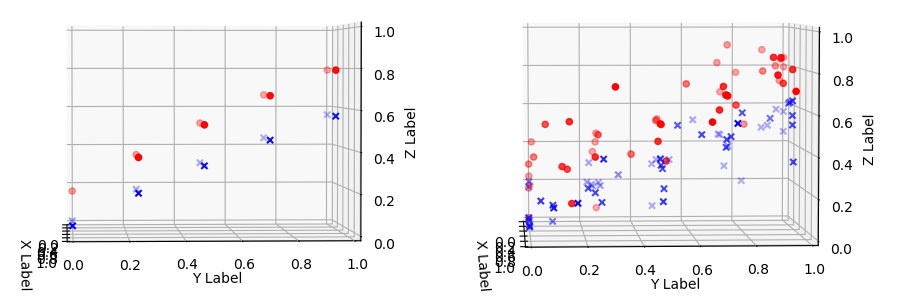
\includegraphics[scale=0.75]{images/metod-images/extend.png}
   \caption{Left graph is pre-data extension, right is post-data extension. The pre-data extension is clearly linearly separable, while the post-data extension is not. }
   \label{fig:extend}
\end{figure}

The BMI data set used in this thesis originates from the original Hyperplane Folding paper. In \cite{unpublished}, an additional 25 points where created per existing point in order to make the BMI data set non-linear. This is reproduced in this thesis, where spherical coordinates is randomized, creating a cloud of points around the original data points. This method is illustrated in Figure \ref{fig:extend}.



\subsection{Feature normalization}
Data scaling is a data pre-processing technique which normalizes the values of the data points in the data set between a given interval \cite{featurescaling-org}. Feature normalization is needed for Support vector machines the accuracy of the model is dependent on they scale of the input data \cite{featurescaling-svm}. Feature normalization improves classification accuracy for some data sets \cite{featurescaling-br} and that Support Vector Machines operates optimally if all vectors are of the same size\cite{1077809}. And as such, all data sets will be be normalized with Linear scaling. This is done by applying a linear search for the smallest value per feature, creating a vector $V_{\text{min}}$. Where for each value $v_i$ in $V$, $v_i$ is the smallest value for $i$ in the data set. The same process is repeated but for the biggest value, creating $V_{\text{max}}$. As subtracting $V_{\text{min}}$ from each point in the data set and dividing it with $V_{\text{max}}$, clamping all values between $[0,1]$. The normalization equation for each point is summarized in \textit{equation} \ref{eq:normalize}. 
\begin{equation}\label{eq:normalize}
\begin{aligned}
     \cfrac{P - V_{\text{min}}}{{V_\text{max}}}
\end{aligned}
\end{equation} 

\par A prerequisite for Hyperplane folding is that data is linearly separable when performing folds since the algorithm utilize hard margin SVMs. If a data set is almost separable it may be applicable to a soft-margin SVM. If so then the data set can be \textit{cleaned} into a separable data set that can be learned from by a hard margin SVM.

\subsection{Data pruning}
In order to make none linearly separable data sets linearly separable, a pruning pre-process was performed, where a soft margin support vector machine is employed on the data set. As soft margin support vector machines allows for some leniency on data points residing inside the margin and even on the wrong side of the decision function, it is able to classify none linearly separable data sets. If the points residing within the margin are identified and pruned, the data set becomes linearly separable.\par
Finding and pruning the outliers is done by classifying all of the training data on the soft margin support vector machine. Since all labels are available for these points, classifying these points and comparing  labels returned by the classifier and actual label are the same. If not, the data set is not linearly separable due to the point, and it is pruned from the data set. Repeating this process for all training data, the data set becomes linearly (hard margin) separable during training phase, thus enabling the usage of Hyperplane folding. The amount of pruning is done by adjusting the \textit{C}-parameter of the Support vector which classifies the training data. Data pruning is visualized in Figure \ref{fig:prune}, where in the left graph, blue points are mixed with red. While post pruning, red and blue data sets are disjointed by the decision function (plane which splits the sets).

\begin{figure}
\centering
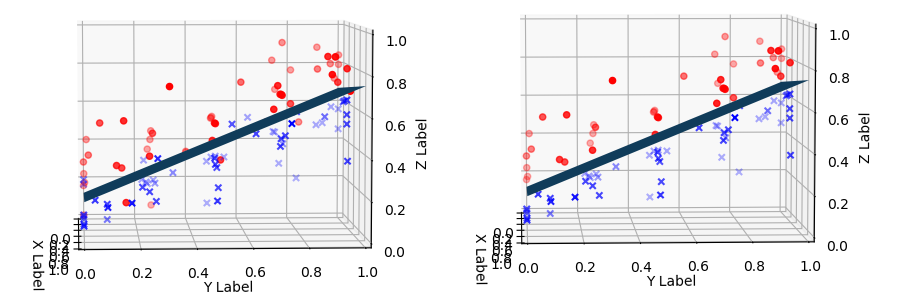
\includegraphics[scale=0.75]{images/metod-images/clean.png}
   \caption{Left graph is pre-data pruning, right is post-data extension. The pre-data extension is clearly not linearly separable, while the post-data extension is linearly separable due to pruning. }
   \label{fig:prune}
\end{figure}

\section{Experiment}

\begin{figure}
\centering
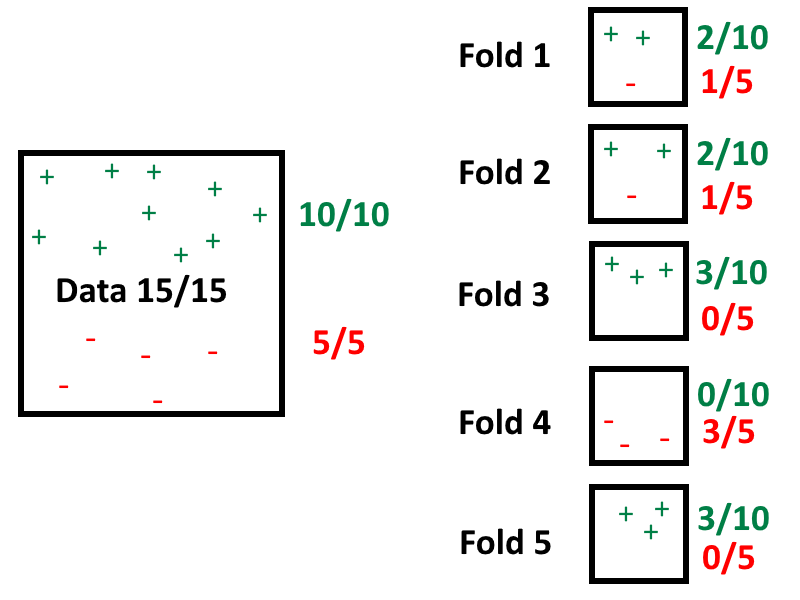
\includegraphics[scale=0.5]{images/metod-images/kfold_normal_fold.png}
   \caption{Non-stratified 5-fold}
   \label{fig:extend}
\end{figure}

\begin{figure}
\centering
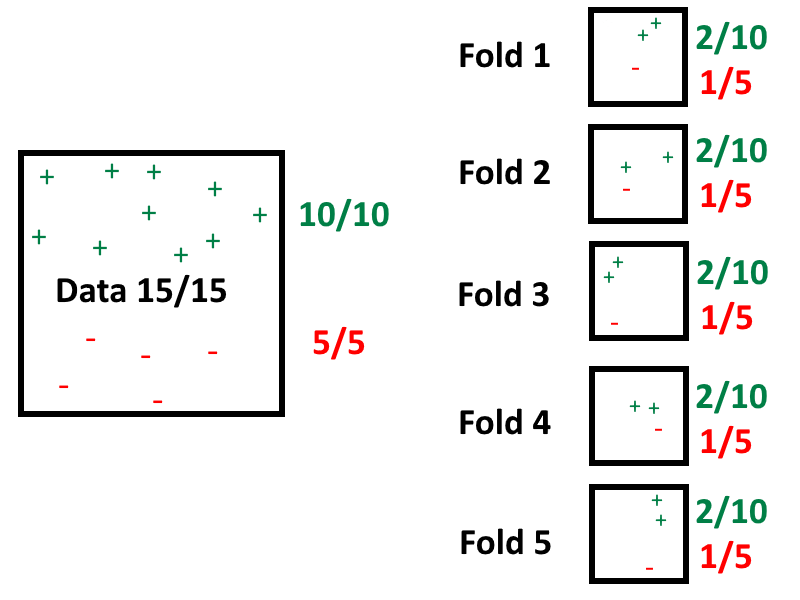
\includegraphics[scale=0.55]{images/metod-images/kfold_stratified_fold.png}
   \caption{Stratified 5-fold}
   \label{fig:extend}
\end{figure}

\subsection{Data sets}
Rubberband folding and Hyperplane folding will be evaluated by using 4 different data sets. Where 
The data sets used for this research question is the BMI \cite{unpublished}, Liver \cite{Dua:2019}, Hepatitis \cite{Dua:2019}, and Breast cancer \cite{breastcancer} data set. \par
The BMI data set is has 3 features and 40 samples. It is used in order to establish a baseline when comparing Hyperplane folding and Rubberband folding, as intial testing in the original Hyperplane folding
paper \cite{unpublished} used it. \par
The other data sets where chosen due to their range of features, the liver data set having 7 features, hepatitis 20 and breast cancer 30. The breast cancer data set where choosen due to its popularity, with atleast 43 citations \cite{Dua:2019}. \par

\subsection{Research question  one}
In order to answer research question 1, how the margin is affected by Rubber band folding will be answered by measuring the margin pre-Rubberband folding (Support vector machine value-margin) and post-Rubberband folding. As Rubberband folding aims at improving Hyperplane folding, its margin will also be collected and compared to Rubberband folding. The model with highest margin is the highest is the best classifier in this category. This will be done by measuring the margin from the data sets when collecting data for Research Question 2.

\subsection{Research question two}
Classification accuracy will be measured by partitioning the data sets into two parts, training and testing. The training set and testing set will be partition by a percentage, where the training data will hold the majority of the data points. As the classification accuracy of the testing set is affected by the accuracy of the classifier (created from training data). The data set is divided into 10-subsets, all of equal size and similar class balance as the entire data set. Where one subset is 10\% of the whole data set. This enables a process where one of these subsets is used for as testing data, and the other ten are used for training. Reapting this process 10 times yields data accuracy as if a larger data pool where available. This simulation is traditionally referred to as Stratified \textit{k}-fold \cite{Flach:2012:MLA:2490546, Japkowicz:2011} or Stratified Cross validation, where \textit{k} is the amount of times the simulation is repeated, normally 5 or 10 times. Our experiment will use 10-fold.
\par Accuracy is the classifiers performance measurement when assigning a class or label to a unknown data (where no data label is available) point. The choice of 10 is due to 10-fold is the optimal choice when sampling classification accuracy, regardless of how much computational power is available\cite{Kohavi:1995:SCB:1643031.1643047}. As Rubber band folding is constrained to the binary classification case, where labels are either true or false. Which in turn leads two 4 possible outcomes when labeling a data point, True Positive (TP, correctly labeling a point as "true"), True Negative (TN), False Positive (FP, incorrectly labeling a a point as False) and False Negative, FN \cite{Japkowicz:2011}. For each data set, a confusion matrix will be presented, with labeling outcomes from all three classifiers. From which Accuracy \ref{eq:accuracy}, True-positive rate \ref{eq:truepositive} and False-negative rate \ref{eq:truenegative}.
\begin{equation}\label{eq:accuracy}
\begin{aligned}
     \cfrac{TP + TN}{TP + TN + FP + FN}
\end{aligned}
\end{equation} 
\begin{equation}\label{eq:truenegative}
\begin{aligned}
     \cfrac{TN}{TN + FP}
\end{aligned}
\end{equation} 
\begin{equation}\label{eq:truepositive}
\begin{aligned}
     \cfrac{TP}{TP + FN}
\end{aligned}
\end{equation} 
 Accuracy is the probability of the classifier correctly labeling an unknown data point. This metric gives an indication of how well the classifier performs on the given data set. It does not show any information as how well it labels each individual class (True, False). If the data set contains 1000 instances, 900 being false, 100 being true, a classifier which labels everything as false would still receive 90\% accuracy. To solve this problem, each class receives its own accuracy measurement, being True / False-rate in order to avoid  \cite{Japkowicz:2011}.  It is therefore important that the usage of artificially generated data sets are utilized, as their distributions are not effected by such problems.  The margin will be measured by calculating the euclidean length of the weight vector, as the weight vectors length is equal to the length from the decision function to a support vector. \cite{Cortes:1995:SN:218919.218929, Flach:2012:MLA:2490546}. \par From the data generated by the stratified 10-Fold a average will be caculated, for the confunfusion matrix, False-rate accuracy, True-rate accuracy and accuracy. The best classifier will be the classifier that scores highest in terms of accuracy, without taking margin into consideration. If the classifier with highest margin performs better, then the conclusion that higher margin equates higher classification accuracy is reasonable. The used data sets will be Breast Cancer, liver and BMI.  \par
Research question two, will be answered by comparing the new technique Rubber band folding with the existing Hyperplane folding, with classification accuracy as metric. 
\begin{equation}\label{eq:risk}
    \cfrac{1}{m}\sum_{i=0}^{m} L(y_i, f(x_i))
\end{equation}
\subsection{Research question three} How the execution time is affected by Hyperplane folding will be answered by measure total execution of the two phases (training and classification) in nano seconds. This is done capturing the time of the day when starting the phase and capturing when the phase is over. The difference between these stamps will be the execution time. 






\chapter{Results and Analysis}
\section{Research Question One}

Data from each data set is presented with a confusion matrix per classifier, being Support Vector Machine (SVM), Hyperplane Folding (HPF) and Rubber band Folding (RBF). The confusion matrix illustrates the distribution of the four possible classifications. A True Positive classification is placed in row True (1) and column (1). A False Negative classification is placed in row True, (1) and column False (2). All correct classifications will be found in the diagonal of the matrix, (1,1) and (2,2). Data entries in the matrices are average results from K-fold iterations. The True-positive rate in Equation \ref{eq:truepositive} and True-negative rate in Equation \ref{eq:truenegative} is calculated from the data presented in these tables. Ideal result is all predictions being found in the diagonal line. \par
Support vector machine's accuracy will not increase per each fold, as it serves a starting point Hyperplane and Rubberband folding, and does not perform any folds.

\clearpage
\FloatBarrier

\section{Results}
\subsection{BMI data set}

\FloatBarrier
\subsubsection{Accuracy}



\begin{figure}[!htb]
\centering
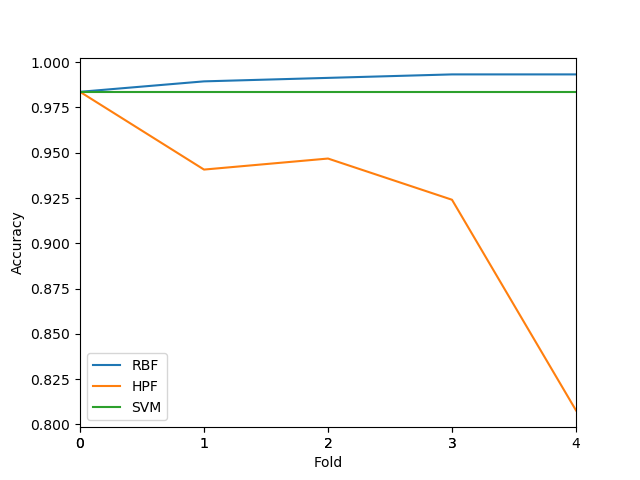
\includegraphics[scale=0.7]{images/result-bmi/Accuracy.png}
   \caption{Figure showing the accuracy for all classifiers over three folds.}
   \label{fig:bmi-accuracy}
\end{figure}

\FloatBarrier

\subsubsection{Analysis}
The accuracy for the classifiers in figure \ref{fig:bmi-accuracy} shows that Rubberband folding outperforms Hyperplane folding with substantial margin. After four folds the difference between Rubberband and Hyperplane folding is $0.993269230769231 - 0.807692307692308 = 0.185576923077$. Rubberband foldings accuracy is higher than Support vector by $0.993269230769231 - 0.983653846153846 = 0.00961538461538$ after four folds. Rubber band folinds accuracy remains unchanged between fold three and four. 

\clearpage
\FloatBarrier

\subsubsection{Specificity}
\begin{figure}[!htb]
\centering
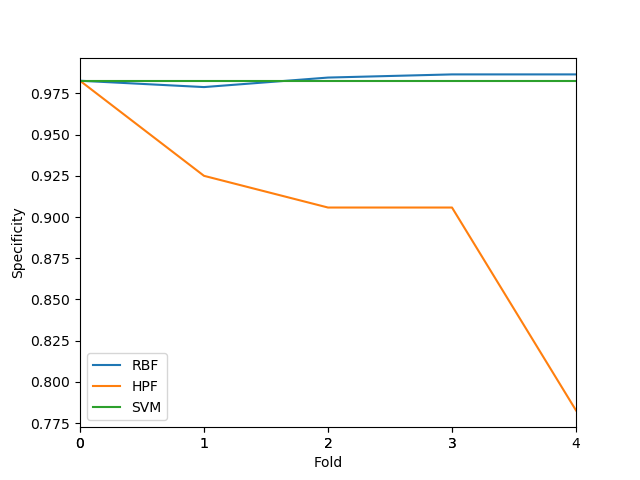
\includegraphics[scale=0.7]{images/result-bmi/Specificity.png}
   \caption{Figure showing the specificity for all classifiers over three folds.}
   \label{fig:bmi-Specificty}
\end{figure}

\FloatBarrier

\subsubsection{Analysis}
Specificity  in \ref{fig:bmi-Specificty} shows that Rubberband folding outperforms all other classifiers after three folds and achieves its highest accuracy after four folds. As the difference between Rubberband fodling and Support vector machine is $0.986538461538462 - 0.982692307692308 = 0.00384615384615$ after four folds. The difference between Rubberband and Hyperplane folding after three folds is $0.986538461538462 - 0.782692307692308 = 0.203846153846$.

\clearpage
\FloatBarrier

\subsubsection{Sensitivity}
\begin{figure}[!htb]
\centering
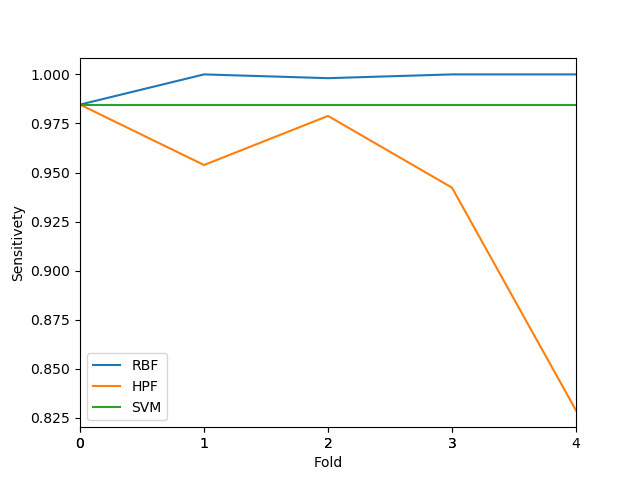
\includegraphics[scale=0.7]{images/result-bmi/Sensitivety.png}
   \caption{Figure showing the sensitiy for all classifiers over three folds.}
   \label{fig:bmi-Sensitivity}
\end{figure}

\FloatBarrier

\subsubsection{Analysis}
Sensitivity in figure \ref{fig:bmi-Sensitivity} shows Rubberband folding reaching 100\% classification rate for positive points after one fold. Hyperplane folding looses sensitivty per each fold. The difference between Rubberband folding and Hyperplane after four folds is $1.0 - 0.828846153846154 = 0.171153846154$. The difference between Rubberband folding and Support vector machine is $1.0 - 0.0153846153846$.

\clearpage

\subsection{Hepatitis data set}

\FloatBarrier
\subsubsection{Accuracy}
\begin{figure}[!htb]
\centering
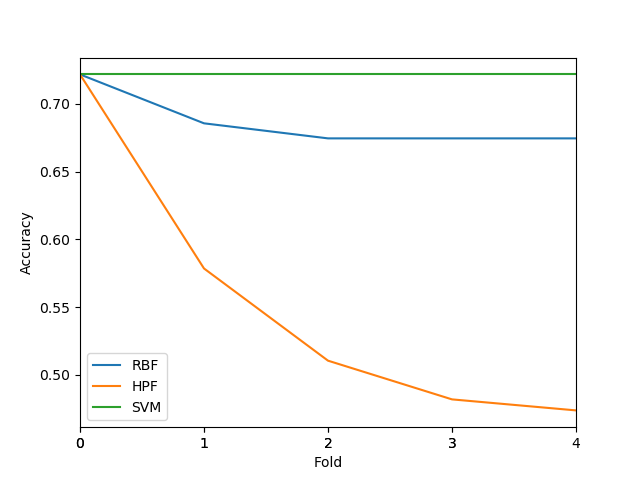
\includegraphics[scale=0.7]{images/result-hep/Accuracy.png}
   \caption{Figure showing the accuracy for all classifiers over three folds.}
   \label{fig:hep-accuracy}
\end{figure}

\FloatBarrier
\subsubsection{Analysis}
Accuracy for Rubberband folding is $0.674603174603175$ compared to Hyperplane foldings $0.473809523809524$ after four folds. Figure \ref{fig:hep-accuracy} shows a steady decline of Hyperplane foldings accuracy, while Rubberband folding decreases from 0.721825396825397 to $0.674603174603175$ after two folds. Neither Rubberband or Hyperplane folding performs better than Support vector machines in overall accuracy. As the difference between Support vector machine and Rubberband foldings accuracy is $0.721825396825397 - 0.674603174603175 = 0.0472222222222 $.\par

\clearpage
\FloatBarrier


\subsubsection{Specificity}
\begin{figure}[!htb]
\centering
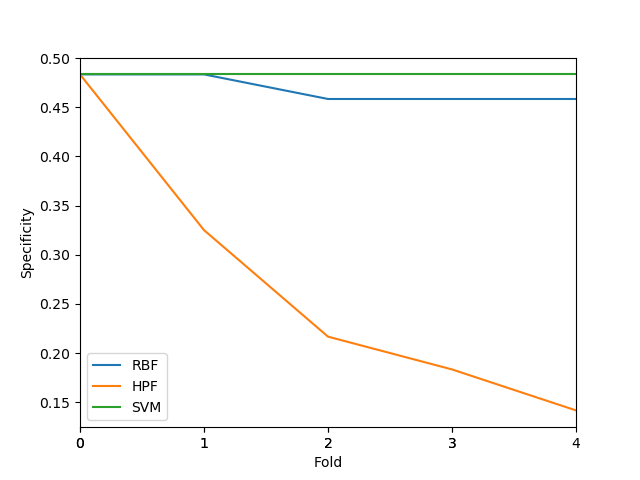
\includegraphics[scale=0.7]{images/result-hep/Specificity.png}
   \caption{Figure showing the specificty for all classifiers over three folds.}
   \label{fig:hep-Specificty}
\end{figure}

\FloatBarrier

\subsubsection{Analysis}
Rubberband folding decreases in specificty after two folds, as it decreases to $0.458333333333333$ from $0.4833333$. This compared to Hyperplane folding where the specificy is $0.141666$ after four folds. The difference between Rubberband folding and Hyperplane folding is $0.4583333 - 0.1416666 = 0.316666663$ after 4 four folds, as seen in figure \ref{fig:hep-Specificty}.

\clearpage
\FloatBarrier

\subsubsection{Sensitivity}
\begin{figure}[!htb]
\centering
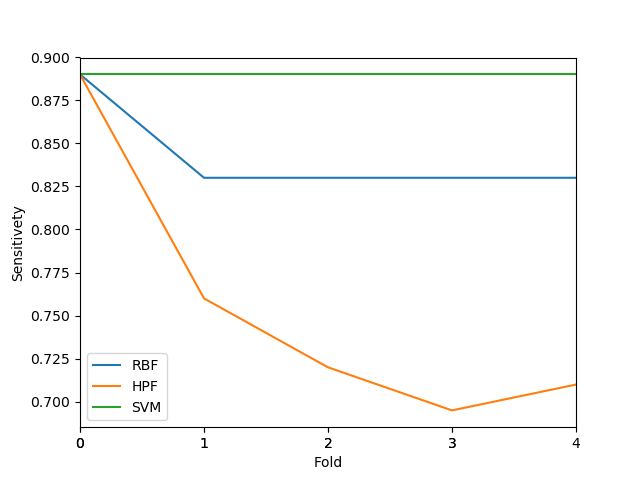
\includegraphics[scale=0.7]{images/result-hep/Sensitivety.png}
   \caption{Figure showing the sensitivity for all classifiers over three folds.}
   \label{fig:hep-Sensitivity}
\end{figure}

\FloatBarrier

\subsubsection{Analysis}
Both Rubberband folding and Hyperplane folding decreases in sensitivity. Hyperplane folding loses sensitivity per each folds, while Rubberband folding looses some sensitivity between the first and second fold. Rubberbands folding sensitivty is the same between fold 2-4. The difference between Rubberband folding and Hyperplane folding is $0.83 - 0.71 = 0.12$ after four folds, as seen in figure \ref{fig:hep-Sensitivity}.

\clearpage
\FloatBarrier

\subsection{Liver data set}
\FloatBarrier
\subsubsection{Accuracy}
\begin{figure}[!htb]
\centering
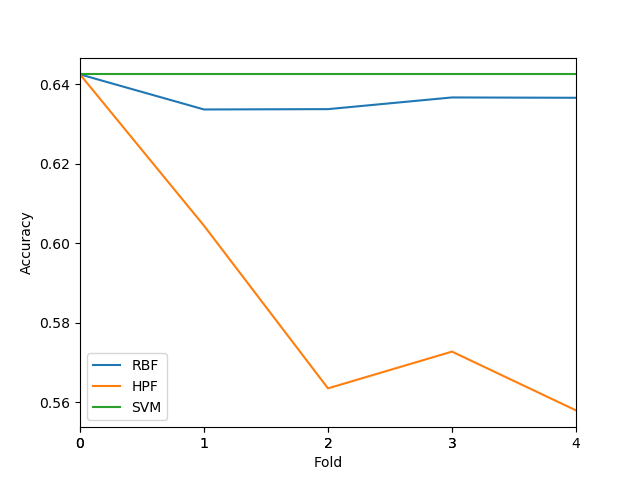
\includegraphics[scale=0.7]{images/result-liver/Accuracy.png}
   \caption{Figure showing the accuracy for all classifiers over three folds.}
   \label{fig:liver-accuracy}
\end{figure}

\FloatBarrier
\subsubsection{Analysis}
Rubberbands accuracy is higher when compared to Hyperplane foldings after four folds. As the difference between Rubberband folding and Hyperplane folding is $0.636638655462185
- 0.557983193277311 = 0.0786554621849$. Rubberbands folding accuracy decreases per each fold, the difference between Support vector machine and Rubberband folding after four folds is, $0.642521008403361 - 0.636638655462185 = 0.00588235294118$, as seen in figure \ref{fig:liver-accuracy}. 

\clearpage
\FloatBarrier
\subsubsection{Specificity}
\begin{figure}[!htb]
\centering
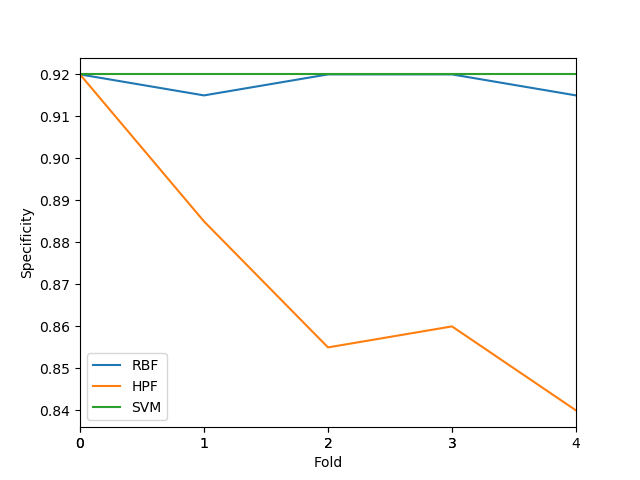
\includegraphics[scale=0.7]{images/result-liver/Specificity.png}
   \caption{Graph illustrates the Specificity for each classifier per fold. SVM Specificity remains the same unchanged, it does not perform any folds, and serves as baseline for the experiment.}
   \label{fig:liver-Specificty}
\end{figure}

\FloatBarrier

\subsubsection{Analysis}
Rubberbands specificity is higher than Hyperplane foldings, as the difference between them is $0.915 - 0.84 = 0.075$ after four folds. Rubberband foldings specificty fluctuate between folds, going from $0.92$ to $0.915$, while Hyperplane folding is decreasing in specificty per fold, as seen in figure \ref{fig:liver-Specificty}.

\clearpage
\FloatBarrier

\subsubsection{Sensitivity}
\begin{figure}[!htb]
\centering
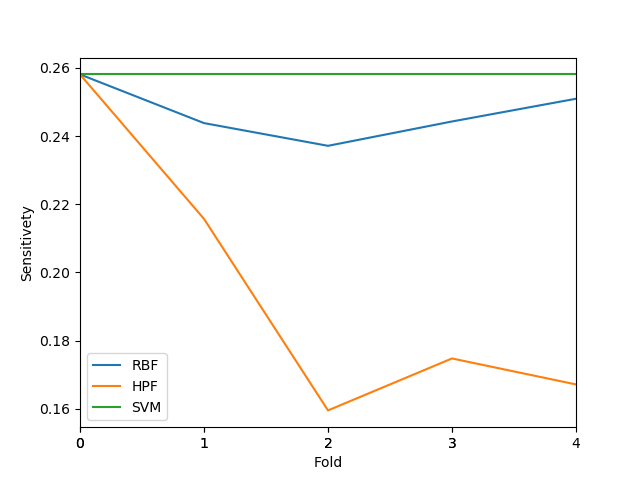
\includegraphics[scale=0.7]{images/result-liver/Sensitivety.png}
   \caption{Figure showing the sensitivty for all classifiers over three folds.}
   \label{fig:liver-Sensitivity}
\end{figure}

\FloatBarrier

\subsection{Analysis}
Rubberband folding decreases in sensitivity between fold 1-2, and regains sensitivty between fold 3-4. The difference between Support vector machine and Rubberband folding after four folds i $0.258095238095238 - 0.258095238095238 = 0.00714285714286$. Rubberband folding decrease in sensitivity between folds 1-2 and again between fold 3-4. The difference between Rubberband folding and Hyperplaen folding after four folds is $0.250952380952381 - 0.167142857142857 = 0.0838095238095$, as seen in figure \ref{fig:liver-Sensitivity}.

\clearpage
\FloatBarrier
\subsection{Breast cancer data set}
\subsubsection{Accuracy}
\begin{figure}[!htb]
\centering
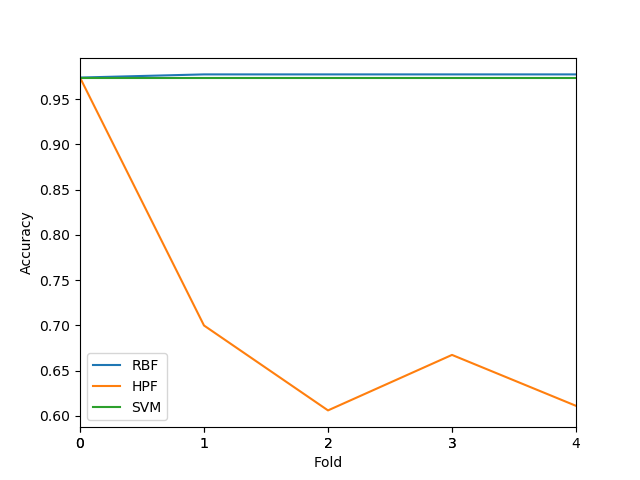
\includegraphics[scale=0.7]{images/result-cancer/Accuracy.png}
   \caption{Figure showing the accuracy for all classifiers over three folds.}
   \label{fig:cancer-accuracy}
\end{figure}

\FloatBarrier
\subsection{Analysis} 
Rubberband folding increases the accuracy to $0.97722106991617$ after one fold. The differece between the Rubberband folding and Support vector machine after one fold is $0.97722106991617 - 0.973742546020223 = 0.00347852389595$. Hyperplane folding decreases in accuracy between folds 1-2 and 3-4. The difference between Rubberband folding and Hyperplane folding after four folds is $97722106991617 - 0.610992999740731 = 0.366228070175$, as seen in figure \ref{fig:cancer-accuracy}
.
\clearpage
\FloatBarrier

\subsubsection{Specificity}
\begin{figure}[!htb]
\centering
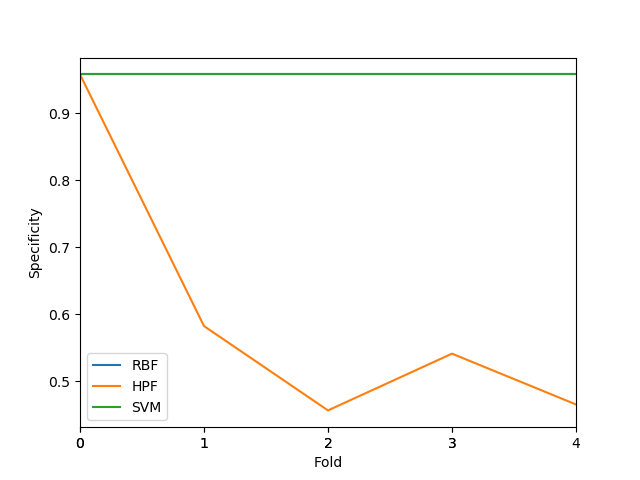
\includegraphics[scale=0.7]{images/result-cancer/Specificity.png}
   \caption{Figure showing the specificty for all classifiers over three folds.}
   \label{fig:cancer-Specificty}
\end{figure}

\FloatBarrier
\subsection{Analysis}
Rubberband foldings specificity remains unchanged during all four folds. the two is $0.957575757575757 - 0.957575757575757 = 0.0$. Hyperplane folding reduces accuracy between fold 1-2 and 3-4. The difference between Rubberband folding and Hyperplane folding after four folds is $0.957575757575757 - 0.465367965368 = 0.492207792208$, as seen in figure \ref{fig:cancer-Specificty}.

\clearpage
\FloatBarrier

\subsubsection{Sensitivity}
\begin{figure}[!htb]
\centering
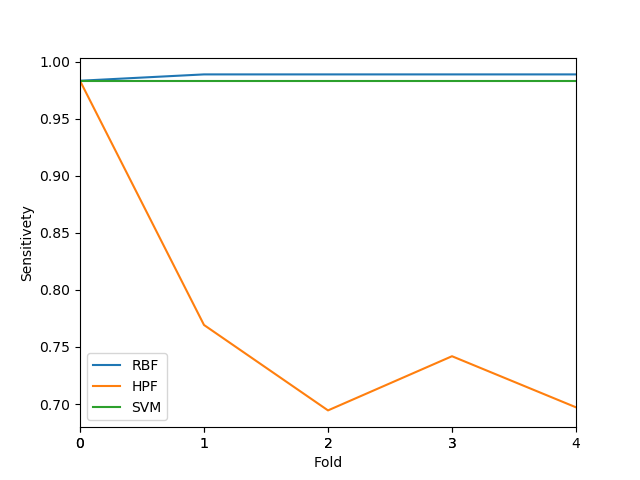
\includegraphics[scale=0.7]{images/result-cancer/Sensitivety.png}
   \caption{Figure showing the sensitivty for all classifiers over three folds.}
   \label{fig:cancer-Sensitivity}
\end{figure}

\FloatBarrier

\subsubsection{Analysis}
Rubberband folding increases the sensitivty after the first fold. The sensitivity remains unchanged between fold 2-4. The sensitivy was increased with $0.988809523809524 - 0.983253968253968 = 0.00555555555556$. Hyperplane folding decreases sensitivity between folds 1-2 and 3-4. The difrecence between Rubberband folding and Hyperplane folding after four folds is $0.988809523809524 - 0.697142857142857 = 0.291666666667$, as seen in figure \ref{fig:cancer-Sensitivity}.

\clearpage
\FloatBarrier



\section{Research Question Two}
 Support vector machine margin will not increase between folds, as it serves as starting point for Rubberband and Hyperplane folding. Same data sets are used for this research question as the previous one. 

\FloatBarrier


\subsection{Margin}
\subsubsection{BMI dataset}
\begin{figure}[!htb]
\centering
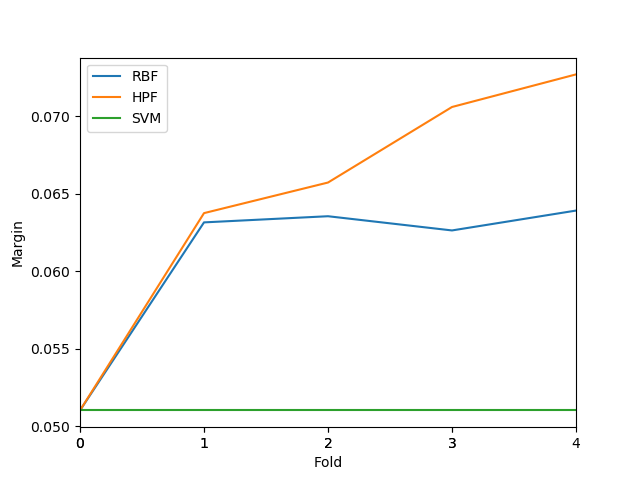
\includegraphics[scale=0.7]{images/result-bmi/Margin.png}
   \caption{Margin over three folds for the classifiers for the BMI dataset}
   \label{fig:bmi-margin}
\end{figure}

\FloatBarrier

\subsubsection{Analysis BMI}
In figure \ref{fig:bmi-margin}, Rubberband and Hyperplane folding increases the margin in the Support vector machine for the BMI dataset. Hyperplane folding achieves a higher margin. Hyperplane folding increases the margin in all for folds. Rubberband folding increases the margin between folds 1-2 and 3-4. The margin decreases with $0.0635435443729617 - 0.0626268152101499 = 0.000916729162812$ Hyperplane folding achieves the highest margin as the differnce between Hyperplane folding and Rubberband folding is $0.0726956327616554 - 0.0639081660051451 = 0.00878746675651$. 

\clearpage
\FloatBarrier
\subsubsection{Hepatitis dataset}
\begin{figure}[!htb]
\centering
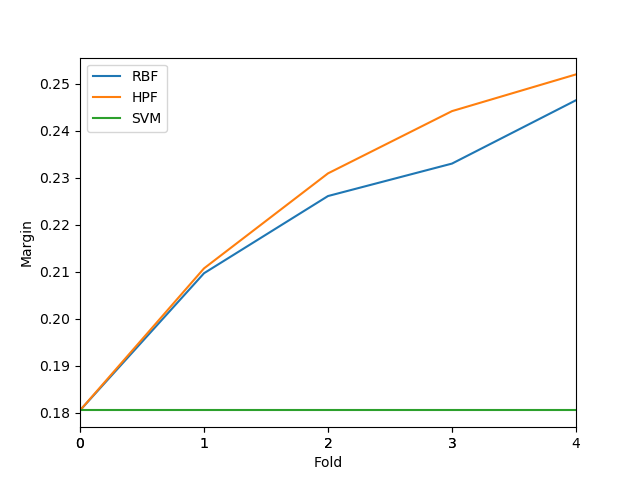
\includegraphics[scale=0.7]{images/result-hep/Margin.png}
   \caption{Margin over three folds for the classifiers for the Hepatits dataset}
   \label{fig:hep-margin}
\end{figure}

\FloatBarrier

\subsubsection{Analysis Hepatitis}
Both Rubberband and Hyperplane folding increases the margin in all folds, as seen in figure \ref{fig:hep-margin}. Hyperplane folding achieves a margin which is $0.252032218864919 - 0.246531075385518 = 0.0055011434794$ higher than Rubberband folding.


\clearpage
\FloatBarrier

\subsubsection{Liver dataset}
\begin{figure}[!htb]
\centering
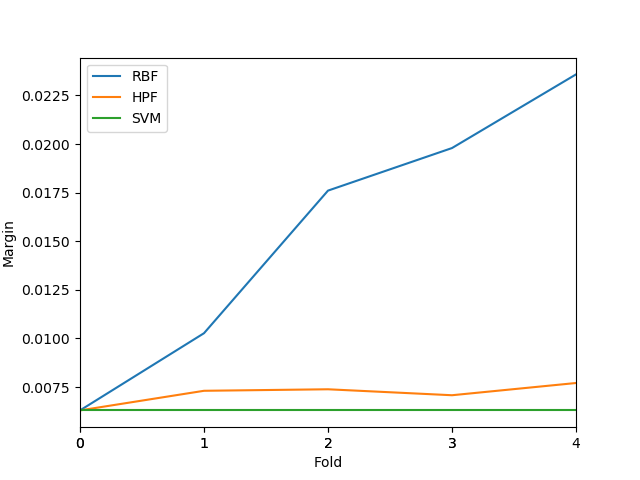
\includegraphics[scale=0.7]{images/result-liver/Margin.png}
   \caption{Margin over three folds for the classifiers for the liver dataset}
   \label{fig:liver-margin}
\end{figure}

\FloatBarrier

\subsubsection{Analysis Liver}
Rubberband folding increases the margin in all four folds. Hyperplane folding increases the margin between 1-2 and 3-4. Rubberband folding increases the margin by $0.0235815958844967 - 0.00629749634302838 = 0.0172840995415$ after four folds. Hyperplane folding increases the margin with $0.00770660161388123 - 0.00770660161388123 =  0.00140910527085$ after the four folds, as seen in figure \ref{fig:liver-margin}.


\clearpage
\FloatBarrier
\subsubsection{Cancer dataset}
\begin{figure}[!htb]
\centering
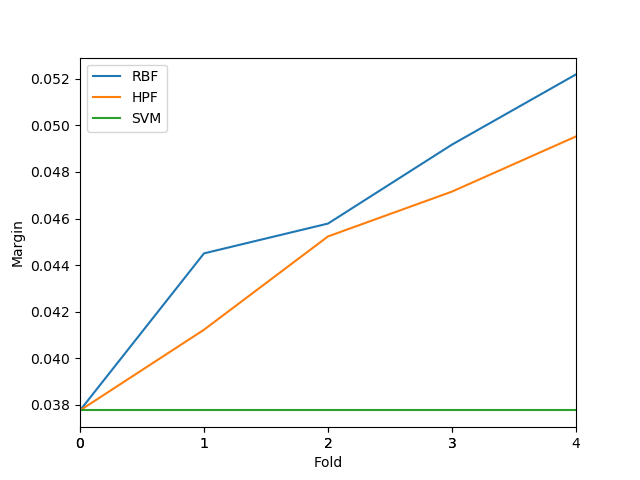
\includegraphics[scale=0.7]{images/result-cancer/Margin.png}
   \caption{Margin over three folds for the classifiers for the Cancer dataset}
   \label{fig:cancer-margin}
\end{figure}

\subsubsection{Analysis Cancer}
Rubberband folding and Hyperplane folding increases the margin in all four folds, as seen in figure \ref{fig:cancer-margin}. Rubberband folding increases the margin by $0.0521849975147187 - 0.0495230091882644 = 0.0144174993406$. Hyperplane folding increases the margin by $0.0495230091882644 - 0.0377674981741026 = 0.0117555110142$. Rubberband folding has the highest margin after for folds.



\clearpage





\section{Research Question Three}
Results are presented in tables and graphs, where each classifiers execution time function is in ms.  Measurements are from all data sets, with varying sample size for training. Support vector machine's execution time for training and classify does not change over folds, as it is a starting point for Rubberband and Hyperplane folding. 
\FloatBarrier

\subsection{Result}

\FloatBarrier

\subsubsection{Classification time}

\begin{figure}[!htb]
\centering
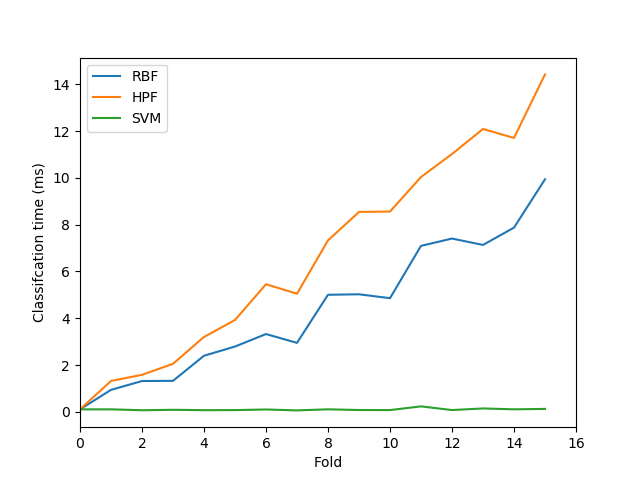
\includegraphics[scale=0.7]{images/result-hep/hep_k_15/Classifcationtime(ms).png}
   \caption{Graph illustrates the classification time in ms, after 15 folds}
   \label{fig:hep-classify}
\end{figure}
\FloatBarrier
\subsubsection{Analysis}
Classification time increases linearly for both Hyperplane folding and Rubberband folding, as seen in figure \ref{fig:hep-classify}. Where Rubberband folding has a lower increase per fold. As the differnece between Hyperplane folding and Rubberband folding is $14.4238 - 9.9398 = 4.484 $ ms after 15 folds. Compared to Support vector machine which classifies the data in $0.1702$ ms. Rubberband folding rotated 349 points, while Hyperplaen folding rotated 500 throughout all 15 folds.\par

\clearpage
\FloatBarrier

\subsubsection{Training time}

\begin{figure}[!htb]
\centering
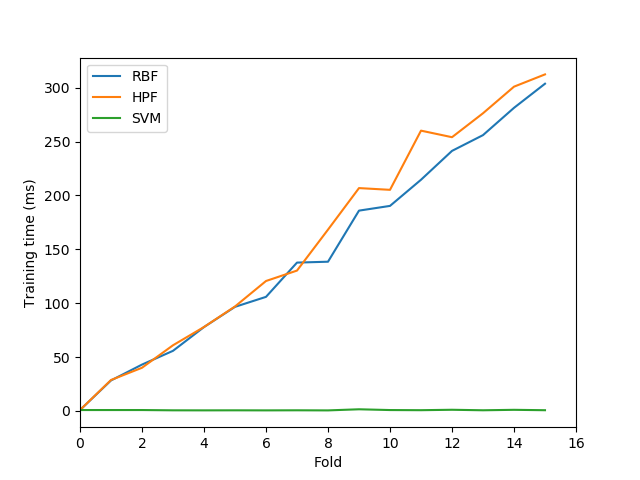
\includegraphics[scale=0.7]{images/result-hep/hep_k_15/Trainingtime(ms).png}
   \caption{Graph illustrates the training time in ms, after 15 folds}
   \label{fig:hep-fit}
\end{figure}
\FloatBarrier
\subsection{Analysis}
Both classifiers increase linearly in training time per fold. Where Rubberband is the slowest during the training phase. As the difference between Rubberband and Hyperplane folding is $312.3823 - 303.7252 = 8.6571$. Support vector machine trains the decision function in $0.7164$ ms.



\chapter{Discussion}
\subsection{Accuracy}
Rubberband folding achieves a higher classification accuracy in all data sets, when compared to Hyperplane folding. This can be attributed to Rubberband folding being affected by over rotation. As Rubberband folding does not rotate data points residing in the zone described in the section \ref{Problem description}. Rubberband increases the overall classification accuracy when applied to the BMI data set by $0.00961538461538$, which corresponds to 0.9\%. This increase is significant, as specificity and sensitivty increases aswell. For example,  an increase in accuracy could stem from sensitivity increasing by 10\%, while specificty decreases by 5\%, which would still lead to net gain in accuracy, albeit misleading. As the increase in accuracy also leads to a decrease when classifying a particular class. Applying this example the breast cancer data set, where classifying 10\% none-benin cancer cells correctly would be of great benefit, while erroneously giving 5\% more patients unnecessary treatment would be unacceptable. As such, the increase in all three accuracy measures for the BMI data indicates that Rubberband folding can increase the classification accuracy. 
\par Rubberbands accuracy does not increase in the Hepatitis data set, instead, a decrease is observed. Overall classification accuracy is decreased by $0.047222222222$. Hyperplane folding has a larger decrease in accuracy. This can be attributed to Rubberband folding not over rotating points. But as Rubberband decreases in specificty and sensitivty, it is not possible draw a conclusion from the data as to why it performs better than Hyperplane folding for hepatitis data set. 
\par Rubberband performs better than Hyperplane folding by a large margin when applied to the liver data set. But does not achieve a accuracy higher than the Support vector machine baseline. Rubberbands behavior differs in the liver data set compared to the hepatitis data set, as the loss of accuracy is not consequent. Rubberband folding regains some accuracy between fold 2-3. This is due to both sensitivty and specificty in figures \ref{fig:liver-Specificty} \ref{fig:liver-Sensitivity} increasing. The exact reasons to why Rubberband folding exhibits such behavior is outside of the scope of this thies \todo{Är det verkligen det???}. \par
Rubberband folding increases the accuracy in the Breast cancer data set, by $0.00347852389595$. This increase is due to sensitivty increasing. Meaning the classifiers ability to correctly detect none-benin cancer cell increases by 0.3\%. This is significant as no decrease in specificty is observed, and as in the BMI dataset, a true increase accuracy without drawback is achieved. Such increase corresponds to correctly detecting none-benin cancer cells in three out of thousand.

\subsection{Margin}
Rubberband folding increases the margin in all data sets in every fold with the exception second fold in the BMI data set. Where the margin decreases with $0.000916729162812$. The loss of margin is can not be attributed to floating point precision error, as the floating point representation throughout this thesis is float64. Meaning that the decline in margin is due to a unhandled corner case in the algorithm, triggered by the bmi data set. The loss of margin is not substantial, and the classification accuracy increases during the same fold, as seen in figure \ref{fig:bmi-accuracy}. Rubberband margin after four folds is higher than Hyperplane folding in the breast cancer and liver data set, albeit lower in the BMI data set and heptitis. The margin increase in the liver data set is substantial, this is due to..... VULLE KOLLA HÄR OCH SKJUT IN NÅGOT SMART.

\subsection{Execution time}

Reults from figure \ref{fig:bmi-classify} indicates that both Rubberband folding and Hyperplane folding increases in execution time when the folds are increased. Where Rubberband folding increases less per fold. This can be attributed to Rubberband folding rotates less points as split plane encapsulates less area and points. This increased over several folds will lead to less points being rotated over time. The almost overlapping lines in figure \ref{fig:hep-fit} indicates that both classifiers takes the same amount of time when training the decision function for data sets. There some variance between the Hyperplane and Rubber band folding, this can be attributed to scheduling of the operating system.

\par The 2D-projection algorithm turned out to be useful for just visualization purposes. Ploting a SVM with a high dimensional feature space is hard to show on a computer screen. With a 2D-projection, a more accurate way of displaying the SVM is possible. This finding is in it self very useful, for not only hyperplane folding.

\chapter{Conclusions}
\section{RQ1}
Rubber band folding increases the margin. So does the Hyperplane folding. It is unclear if Rubberband folding increases the margin more than Hyperplane folding for a given set. Depending on the nature of the data RBF made larger increase in margin
\section{RQ2}
Rubberband folding can increase the classification accuracy, where both specificty and sensitivy increases, causing a true increase in accuracy. For most training data used for testing during the thesis, the accuracy decreases. The accuracy for HPF using RBF contrary to not using RBF is always better. What type of data and when it is suitable to use HPF with RBF over a standard SVM is at this state of development unclear. 

\section{RQ3}
Rubberband and Hyperplane folding exhibits linear behavior when the amount of folds increases, for both classification and training. Rubberband folding classifies data points faster when the amount of folds increases, as it rotates less points. 

\chapter{Future Work}
\par Rotations are technically applicable in any dimension. Theoretically Hyperplane folding should be applicable in any dimension, that is without the need of a 2D-projection. The projection in itself serves as a great tool for visualizing SVMs of any dimension. How ever, the main purpose of the projection was to ensure control when performing the folds. Thinking in two dimensions are easier compared to higher dimensions. An investigation in performing Hyperplane folding in the datas original dimensionality is something for the future. This would also yield a performance increase as the calculation of the projection matrix would be unnecessary.

\par Rubber band folding was this thesis attempt at solving some of Hyperplane foldings weaknesses. There may be better ways that eliminate more of its problems. There are not to much related work on the subject and a lot of RBFs properties has been made up iteratively during the progression of the thesis.

\par State of the art SVMs are built to handle more than binary data. Much like the first method proposed by Vapnik \cite{Cortes:1995:SN:218919.218929, vapnik1} Hyperplane folding requires the data to be binary. Building the Hyperplane folding algorithm to handle multi-class problems would be desirable for common applications.

\par Hyperplane folding is bound to being a hard-margin SVM. More extensive experiments with methods to make data linearly separable using kernels and data pruning could improve the current state of the algorithm. Researching a way of using soft-margin SVMs instead hard-margin SVMs could yield a Hyperplane folding algorithm that could be run directly on inseparable data.

\par Not much have been said about Hyperplane foldings time complexity in this thesis. Folds and rotations takes performance. The 2D-projection scales away a lot of performance and could be measured for better metrics.

\par After folding, the data points may not be normalized any more. SVMs perfer to have its training data normalized. Therefore an investigation in keeping the relation between points post folding could be conducted. 


% All references are in a separate file: thesis-refs.bib
\bibliography{thesis-refs}
\bibliographystyle{plain}

\appendix
\chapter{Supplemental Information}










% DO NOT CHANGE BELOW
% This part makes sure that the last page is even with BTH-logo.
% -------------------
\cleardoublepage
\thispagestyle{empty}
\vspace*{\fill}
\clearpage{\thispagestyle{empty}}
\changepage{3cm}{1cm}{-0.5cm}{-0.5cm}{}{-1.5cm}{}{}{}
\vspace*{\fill}
\center

{\bthcsnotextlogo{3cm}}
\\
\noindent\makebox[\linewidth]{\rule{\textwidth}{1pt}} 
Faculty of \faculty, Blekinge Institute of Technology, 371 79 Karlskrona, Sweden
% -------------------

\end{document}
